\chapter{Instalação e uso do \textit{LSD-SLAM}}

\renewcommand{\tablename}{Listagem}

\section{Instalação da estação de trabalho}

Este capítulo foi incluído para servir de referência aos leitores que desejarem usar a ferramenta \textit{LSD-SLAM} no futuro. Contém algumas informações que consideramos úteis e soluções para alguns dos problemas encontrados.

Etapas para preparação:

\begin{enumerate}
	\item{Instalação do \textit{Ubuntu}: A instalação do \textit{Ubuntu} deve ser da versão 12 ou 14 obrigatoriamente, a versão usada no trabalho foi a 14.04.}
	\item{Instalação do  \textit{ROS}: O \textit{ROS} vai ser utilizado para a leitura dos quadros da câmera/\textit{dataset} além de ser onde a ferramenta é implementada.\cite{ROS-Tutorial}}
	\item{Instalação do \textit{LSD-SLAM}.\cite{GitHub-LSD-SLAM}}
	\item{Instalação do  \texttt{usb\_cam}: \texttt{usb\_cam} é um \textit{driver} \textit{ROS} para habilitar câmeras \textit{USB} a serem utilizadas como \textit{stream} de dados para o \textit{ROS} e consequentemente o \textit{LSD-SLAM}, se não há intenção de usar câmeras, como quando utilizando um \textit{dataset}, o \textit{driver} \textit{USB} não é necessário.}
	\item{Calibração da câmera: Será detalhado nas próximas sessões.}
\end{enumerate}

\section{Calibração da câmera}

Uma calibração da câmera do \textit{OpenCV} pode ser usada no \textit{LSD-SLAM} no entanto ele vem na sua instalação uma ferramenta de calibração mais intuitiva e confiável por oferecer um retorno ao usuário se as amostras tiradas são o suficiente ou não. Além disso câmeras \textit{USB} não podem ser configuradas usando o \textit{software} \textit{Android} \textit{PhotoGuide}.

\subsection{Imprimindo o padrão tabuleiro de xadrez}

Antes de utilizar a câmera deve-se calibrá-la a fim de eliminar a distorção radial que possa ocorrer ao se capturar quadros da mesma forma que no \textit{OpenCV}.
Primeiramente deve-se imprimir um tabuleiro de xadrez \cite{Setup-CalibrateMonocularCamera}, preferencialmente em uma folha ou cartolina A3 ou A4 e fixado em uma superfície rígida e plana. Essa folha não deve: 

\begin{itemize}
	\item{Estar amassada.}
	\item{Coberta com algum material refletor ou fita adesiva em qualquer parte do tabuleiro.}
	\item{Estar com alguma “casa” do tabuleiro cortada por impressão.}
	\item{Estar com tinta esmaecida ou borrada.}
\end{itemize}	

Todos esses fatores interferem no reconhecimento do padrão fazendo com que o resultado da calibração se torne falho. Com o tabuleiro em mãos, tomando cuidado para não cobrir as “casas” do tabuleiro, mova-se para um lugar espaçoso de pelo menos $5m^2$, livre de obstruções e bem iluminado.

\subsection{Compilando e construindo a ferramenta de calibração}

Começa-se obtendo as dependências necessárias e compilando o \textit{driver} usando os seguintes comandos respectivamente:

\begin{table}[H]\label{tb:1}
\begin{tabular}{| p{\textwidth}|}
\hline
\texttt{\$ rosdep install camera\_calibration} \\
\texttt{\$ rosmake camera\_calibration} \\ \hline
\end{tabular}
\caption{Comandos para inicializar a instalação do módulo que fará a calibração da câmera}
\end{table}


\subsection{Envio de quadros pela câmera}

Antes de começar a calibração deve-se concluir configuração do pacote usb\_cam e a câmera deve estar conectada e configurada pelo pacote. Para ter certeza que a câmera está de fato enviando seus dados para o \textit{ROS}, usa-se o seguinte comando:

\begin{table}[H]\label{tb:2}
\begin{tabular}{| p{\textwidth}|}
\hline
\texttt{\$ rostopic list}\\
\hline
\end{tabular}
\caption{Comandos para inicializar a instalação do módulo que fará a calibração da câmera}
\end{table}

Esse comando irá listar todos os \textit{topics} que são os nodos ativos no \textit{ROS}. A saída deve conter esses \textit{topics}:

\begin{table}[H]\label{tb:3}
\begin{tabular}{| p{\textwidth}|}
\hline
\texttt{/usb\_cam/camera\_info} \\
\texttt{/usb\_cam/image\_raw}\\
\hline
\end{tabular}
\caption{Resultado com os \textit{topics}}
\end{table}

Caso a saída não apresente erros, a câmera está pronta para ser calibrada.

\subsection{Rodando o nodo de calibração}

Para começar a calibração é necessário carregar os \textit{topics} com as imagens da câmera que será calibrada usando o seguinte comando:

\begin{table}[H]\label{tb:4}
\begin{tabular}{| p{\textwidth}|}
\hline
\texttt{\$ rosrun camera\_calibration cameracalibrator.py --size 9x6 --square 0.108 image:=/usb\_cam/image\_raw camera:=/usb\_cam}\\
\hline
\end{tabular}
\caption{Inicialização do módulo que calibrará a câmera}
\end{table}

Vale frisar a importância de que o parâmetro \texttt{--size} é o tamanho do tabuleiro, no entanto ele conta não as casas e sim as linhas entre as casas:

\begin{figure}[H]
	\centering
		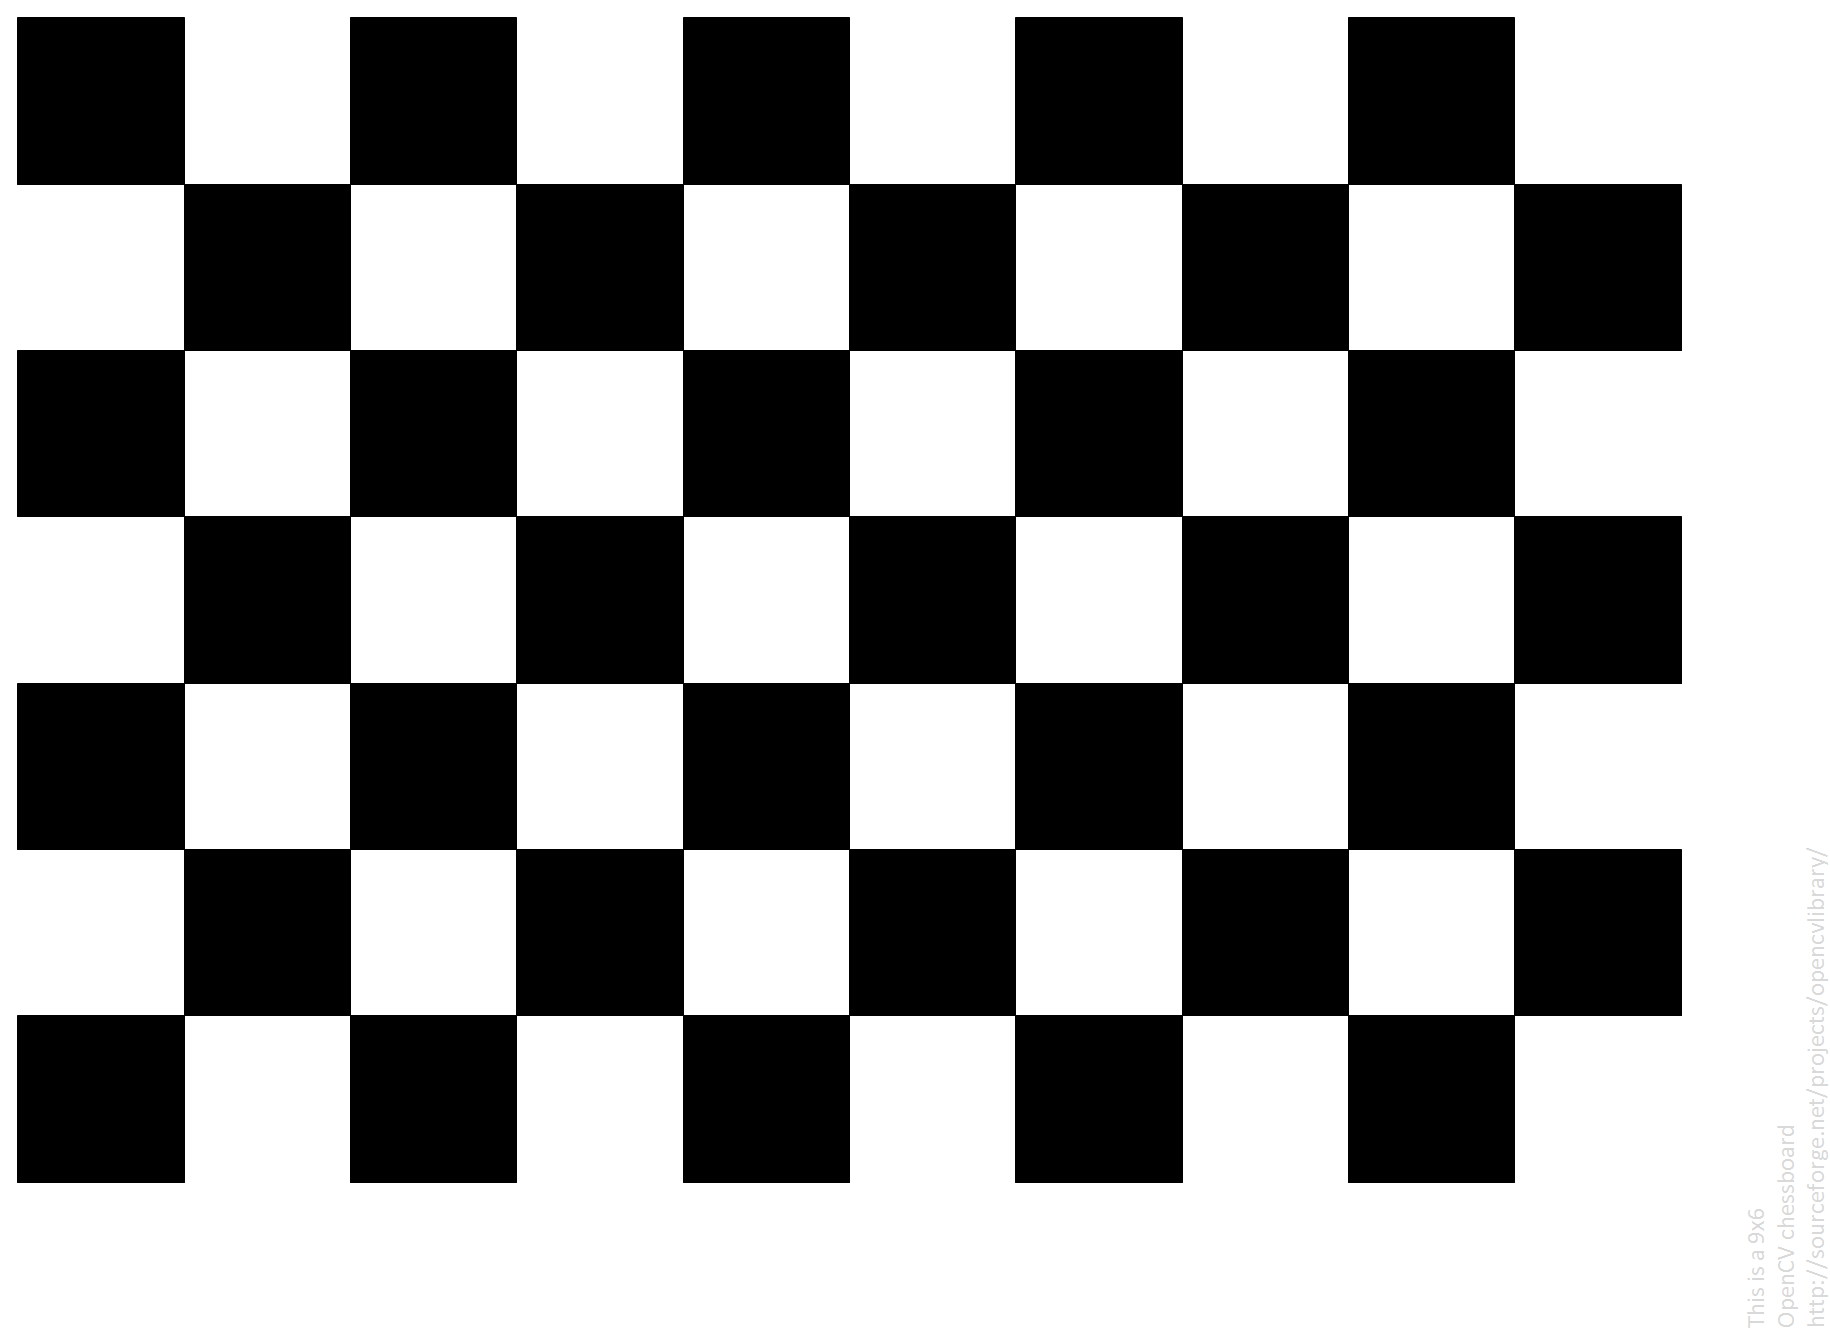
\includegraphics[width= \textwidth]{Imagens/figura3-3E3-12.png}
	\caption{Exemplo de padrão utilizado para a calibração}
	\label{fig3:12}
\end{figure}


Esse padrão por exemplo tem 10x7 casas, no entanto suas linhas são 9x6. Logo o parâmetro \texttt{--size} deve ser 9x6.
O parâmetro \texttt{--square} é o tamanho real do lado das casas do tabuleiro que imprimimos em metros. O comando acima indica que cada casa do tabuleiro possui 0,108 metros ou 10,8 centímetros. É recomendado que o usuário que reproduza estes passos use uma régua para medir o seu tabuleiro.
Após executar o comando, a janela de calibração será aberta, como mostra a figura 3.13:

\begin{figure}[H]
	\centering
		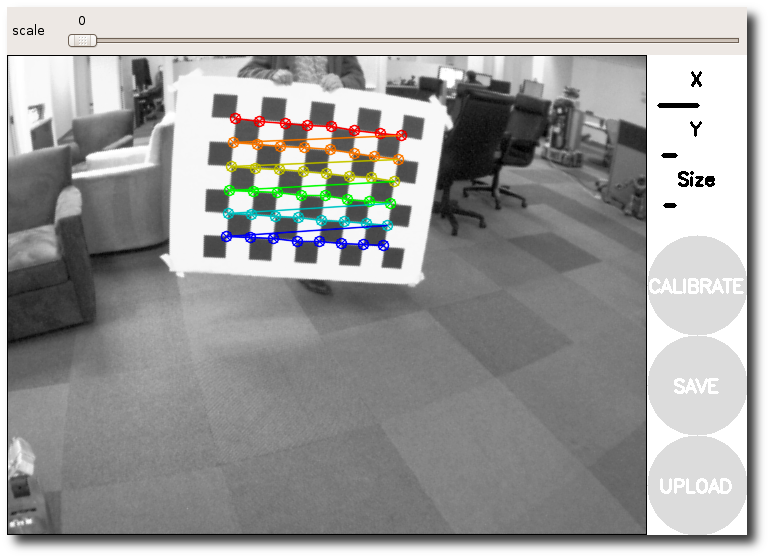
\includegraphics[width= \textwidth]{Imagens/figura3-13.png}
	\caption{Janela de configuração reconhecendo do tabuleiro}
	\label{fig3:13}
\end{figure}

\subsection{Movendo o tabuleiro}

Para se obter uma boa calibração é necessário mover o tabuleiro pelo quadro da câmera de modo que:

\begin{itemize}
	\item{O tabuleiro se encontre nas partes esquerda, direita, superior e inferior do campo de vista da câmera.}
	\begin{itemize}
		\item{Barra X - Campo de vista esquerda/direita.}
		\item{Barra Y - Campo de vista topo/baixo.}
		\item{Barra \textit{Size} - Aproximando/Afastando e Rotação da câmera.}
	\end{itemize}
	\item{O tabuleiro preencha todo o campo de vista.}
	\item{O tabuleiro inclinado para a esquerda,direita,topo,baixo (Barra \textit{Skew})}
\end{itemize}

A cada passo segure o tabuleiro até que que apareça na imagem o destaque do padrão.

\begin{figure}[H]
\minipage{0.32\textwidth}
  \caption{Desmonstração de posição para calibração \#1 \cite{Documentacao-CalibrateMonocularCamera}}\label{fig3:14}
  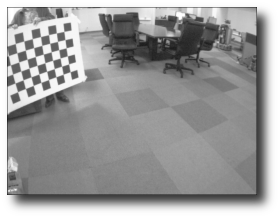
\includegraphics[width=\linewidth]{Imagens/figura3-14.png}
\endminipage\hfill
\minipage{0.32\textwidth}
  \caption{Desmonstração de posição para calibração \#2 \cite{Documentacao-CalibrateMonocularCamera}}\label{fig3:15}
  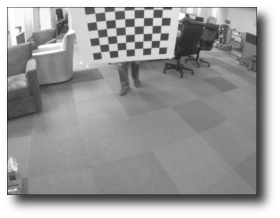
\includegraphics[width=\linewidth]{Imagens/figura3-15.png}
\endminipage\hfill
\minipage{0.32\textwidth}
  \caption{Desmonstração de posição para calibração \#3 \cite{Documentacao-CalibrateMonocularCamera}}\label{fig3:16}
  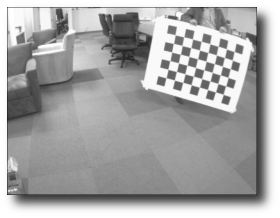
\includegraphics[width=\linewidth]{Imagens/figura3-16.png}
\endminipage
\end{figure}

\begin{figure}[H]
\minipage{0.32\textwidth}
  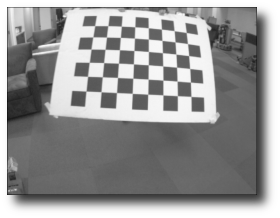
\includegraphics[width=\linewidth]{Imagens/figura3-17.png}
  \caption{Desmonstração de posição para calibração \#4 \cite{Documentacao-CalibrateMonocularCamera}}\label{fig3:17}
\endminipage\hfill
\minipage{0.32\textwidth}
  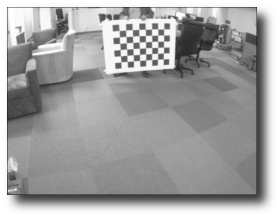
\includegraphics[width=\linewidth]{Imagens/figura3-18.png}
  \caption{Desmonstração de posição para calibração \#5 \cite{Documentacao-CalibrateMonocularCamera}}\label{fig3:18}
\endminipage\hfill
\minipage{0.32\textwidth}
  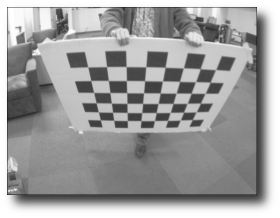
\includegraphics[width=\linewidth]{Imagens/figura3-19.png}
  \caption{Desmonstração de posição para calibração \#6 \cite{Documentacao-CalibrateMonocularCamera}}\label{fig3:19}
\endminipage
\end{figure}

Ao mover o tabuleiro, podem ser percebidas 4 Barras: X,Y,\textit{Size},\textit{Skew}; na barra lateral que aumentam de tamanho conforme ele vai capturando amostras. Quando o botão \textit{CALIBRATE} estiver iluminado quer dizer que há dados suficientes para calibrar. Um clique no botão inicia o processo de calibração.
A calibração dura em média um minuto. A janela estará cinza e inativa durante esse tempo. Isso indica que a calibração está ocorrendo e o programa não travou, bastando apenas aguardar.

\subsection{Resultados da calibração}

Depois de concluída a calibração os resultados dessa calibração podem ser vistos no terminal como demonstra a listagem \ref{tb:5}. Os valores poderão diferir dos apresentados, dependendo da câmera utilizada:


%{\setlength{\parindent}{0cm}
\begin{table}[H]\label{tb:5}
\begin{tabular}{| p{\textwidth}|}
\hline
\textcolor{orange}{\texttt{D = [-0.33758562758914146, 0.11161239414304096, -0.00021819272592442094, -3.029195446330518e-05]}}\\
\textcolor{orange}{\texttt{K = [430.21554970319971, 0.0, 306.6913434743704, 0.0, 430.53169252696676, 227.22480030078816, 0.0, 0.0, 1.0]}}\\
\texttt{R = [1.0, 0.0, 0.0, 0.0, 1.0, 0.0, 0.0, 0.0, 1.0]}\\
\texttt{P = [1.0, 0.0, 0.0, 0.0, 0.0, 1.0, 0.0, 0.0, 0.0, 0.0, 1.0, 0.0]}\\
 \texttt{\# oST version 5.0 parameters}\\
\\
 \texttt{[image]}\\
\\
\textcolor{orange}{\texttt{width}}\\
\textcolor{orange}{\texttt{640}}\\
\\
\textcolor{orange}{\texttt{height}}\\
\textcolor{orange}{\texttt{480}}\\
\\
 \texttt{[narrow\_stereo/left]}\\
\\
\texttt{camera matrix}\\
\texttt{430.215550 0.000000 306.691343}\\
\texttt{0.000000 430.531693 227.224800}\\
\texttt{0.000000 0.000000 1.000000}\\
\\
 \texttt{distortion}\\
 \texttt{-0.337586 0.111612 -0.000218 -0.000030 0.0000}\\
\\
 \texttt{rectification}\\
 \texttt{1.000000 0.000000 0.000000}\\
 \texttt{0.000000 1.000000 0.000000}\\
 \texttt{0.000000 0.000000 1.000000}\\
\\
 \texttt{projection}\\
 \texttt{1.000000 0.000000 0.000000 0.000000}\\
\\
 \texttt{0.000000 1.000000 0.000000 0.000000}\\
 \texttt{0.000000 0.000000 1.000000 0.000000}\\
\hline
\end{tabular}
\caption{Resultados da calibração impressos no console}
\end{table}

%}


 
Os valores destacados serão utilizados em breve. Uma calibração bem sucedida resultará em linhas retas no mundo real aparecerem como linhas retas na imagem corrigida. Uma calibração falha normalmente resulta em imagens em branco, irreconhecíveis ou que não preservam as linhas retas.
Após uma calibração bem sucedida pode-se ajustar o \textit{slider} \textit{SCALE} no topo da janela de calibração para mudar o tamanho da imagem retificada. Uma escala de 0.0 significa que a imagem está formatada de modo que os \textit{pixels} pretos criados para a preencher os espaços deixados pelos \textit{pixels} movidos não estejam presentes. A imagem não terá as curvas pretas de correção mas alguns \textit{pixels} da imagem original serão descartados. A escala de 1.0 significa que todos os \textit{pixels} da imagem original são visíveis mas a imagem corrigida tem bordas pretas onde não há \textit{pixels} de entrada da imagem original.
Se a calibração for satisfatória, o botão \textit{COMMIT} deve ser clicado para enviar os parâmetros de calibração para o armazenamento permanente. A \textit{GUI} fechará e a seguinte mensagem será impressa no console \textit{“writing calibration data to...”}.

\subsection{Criação do arquivo de calibração}

Do modo que está, o \textit{LSD-SLAM} irá utilizar a calibração salva, no entanto é interessante criar um arquivo de configuração para ser facilmente reutilizado caso se queira usar essa configuração em outra máquina ou salvar a calibração em um local mais seguro. Esse arquivo de calibração também é importante pois o \texttt{dataset\_slam} necessita dele para executar, ou seja, ele não usa a calibração salva pelo calibrador em disco. Na seção anterior foram destacadas em laranja alguns valores:

%{\setlength{\parindent}{0cm}
\begin{table}[H]\label{tb:6}
\begin{tabular}{| p{\textwidth}|}
\hline
\texttt{D = [\textcolor{orange}{-0.33758562758914146}, \textcolor{orange}{0.11161239414304096}, \textcolor{orange}{-0.00021819272592442094}, \textcolor{orange}{-3.029195446330518e-05}]}\\
\texttt{K = [\textcolor{red}{430.21554970319971}, 0.0, \textcolor{purple}{306.6913434743704}, 0.0, \textcolor{blue}{430.53169252696676}, \textcolor{brown}{227.22480030078816}, 0.0, 0.0, 1.0]}\\
\\
\texttt{width}\\
\texttt{\textcolor{OliveGreen}{640}}\\
\\
\texttt{height}\\
\texttt{\textcolor{WildStrawberry}{480}}\\
\\
\hline
\end{tabular}
\caption{Informações relevantes extraídas da listagem \ref{tb:5}}
\end{table}


Esses valores serão usados para compor o arquivo. Em um novo documento de texto insira o seguinte modelo:

\begin{table}[H]\label{tb:7}
\begin{tabular}{| p{\textwidth}|}
\hline
\texttt{\textcolor{red}{fx}/\textcolor{OliveGreen}{width} \textcolor{blue}{fy}/\textcolor{WildStrawberry}{height} \textcolor{purple}{cx}/\textcolor{OliveGreen}{width} \textcolor{brown}{cy}/\textcolor{WildStrawberry}{height} \textcolor{orange}{d}}\\
\texttt{\textcolor{OliveGreen}{in\_width} \textcolor{WildStrawberry}{in\_height}}\\
\texttt{"crop" / "full" / "none"}\\
\texttt{\textcolor{OliveGreen}{out\_width} \textcolor{WildStrawberry}{out\_height}}\\
\hline
\end{tabular}
\caption{Modelo de arquivo de configuração com legenda}
\end{table}

Dessa forma deve-se fazer os cálculos substituindo os valores do modelo com os da suas cores respondentes acima, quanto mais casas decimais, melhor, pois isso potencialmente reduz o erro. Na terceira linha:

\begin{description}
\item[\texttt{crop}]{Corta a imagem para o tamanho máximo enquanto inclui apenas \textit{pixels} válidos.}
\item[\texttt{full}]{Não corta a imagem mas pode incluir \textit{pixels} inválidos}
\item[\texttt{none}]{Não realiza a operação de correção de distorção radial}
\end{description}

Recomenda-se o uso do valor \texttt{crop}. O resultado final deve ficar à listagem \ref{tb:8}:

\begin{table}[H]\label{tb:8}
\begin{tabular}{| p{\textwidth}|}
\hline
\texttt{
0,672211796411249546875 0,89694102609784741666666666666667 0,47920522417870375 0,473385000626642 -0.33758562758914146 0.11161239414304096 -0.00021819272592442094 -0.00003.029195446330518}\\
\texttt{640 480}\\
\texttt{crop}\\
\texttt{640 480}\\
\hline
\end{tabular}
\caption{Exemplo de arquivo de configuração final}
\end{table}

Uma observação é que ao inserir os resultados no arquivo, deve-se certificar que o ponto flutuante é ‘.’(ponto) e não ‘,’(vírgula) pois isso fará com que o arquivo não funcione corretamente. Depois disso arquivo deve ser salvo como \texttt{nome\_do\_arquivo\_de\_calibração.cfg} e estará pronto para ser usado. Se estiver usando um arquivo de calibração do \textit{OpenCV}, que foi o usado no \textit{PhotoGuide}, a transformação é similar ao resultado da calibração do \textit{LSD-SLAM}. Considerando a seguinte saída da calibração do \textit{OpenCV}:

\begin{table}[H]\label{tb:9}
\begin{tabular}{| p{\textwidth}|}
\hline
\texttt{<Camera\_Matrix type\_id="opencv-matrix">}\\
\texttt{<rows>3</rows>}\\
\texttt{<cols>3</cols>}\\
\texttt{<dt>d</dt>}\\
\texttt{<data>}\\
\texttt{ \textcolor{red}{6.5746697944293521e+002} 0. \textcolor{purple}{3.1950000000000000e+002}}\\
\texttt{ 0. \textcolor{blue}{6.5746697944293521e+002} \textcolor{brown}{2.3950000000000000e+002}}\
\texttt{ 0. 0. 1.}\\
\texttt{</data></Camera\_Matrix>}\\
\texttt{<Distortion\_Coefficients type\_id="opencv-matrix">}\\
\texttt{<rows>5</rows>}\\
\texttt{<cols>1</cols>}\\
\texttt{<dt>d</dt>}\\
\texttt{<data>}\\
\texttt{ \textcolor{orange}{-4.1802327176423804e-001 5.0715244063187526e-001 0. 0.} -5.7843597214487474e-001</data></Distortion\_Coefficients>}\\
 \hline
\end{tabular}
\caption{Exemplo de arquivo de calibração do \textit{OpenCV}}
\end{table}

Deve ser convertido para um arquivo no formato \textit{.cfg} de modo que:

\begin{table}[H]\label{tb:10}
\begin{tabular}{| p{\textwidth}|}
\hline
\texttt{\textcolor{red}{fx} \textcolor{purple}{fy} \textcolor{blue}{cx} \textcolor{brown}{cy} \textcolor{orange}{k1 k2 p1 p2}}\\
\texttt{640 480}\\
\texttt{"crop" / "full" / "none"}\\
\texttt{640 480}\\
 \hline
\end{tabular}
\caption{Modelo de arquivo de configuração usando a calibração do \textit{OpenCV}}
\end{table}

Lembrando que o \textit{LSD-SLAM} não suporta notação científica, nesse exemplo o arquivo final ficará dessa forma:

\begin{table}[H]\label{tb:11}
\begin{tabular}{| p{\textwidth}|}
\hline
\texttt{0.065746697944293521 0.03195 0.065746697944293521 0.02395 -0.41802327176423804 0.50715244063187526 0 0}\\
\texttt{640 480}\\
\texttt{crop}\\
\texttt{640 480}\\
 \hline
\end{tabular}
\caption{Exemplo de arquivo de configuração final usando a calibração do \textit{OpenCV}}
\end{table}

\section{Utilização da ferramenta}

Com a câmera calibrada pode-se agora começar a usar de fato a ferramenta. O \textit{LSD-SLAM} é dividido em dois pacotes \textit{ROS}, \texttt{lsd\_slam\_core} e \texttt{lsd\_slam\_viewer}. \texttt{lsd\_slam\_core} contém o sistema \textit{SLAM} completo, enquanto o \texttt{lsd\_slam\_viewer} é opcionalmente usado para a visualização 3D.
Para inicializar o sistema do \textit{LSD-SLAM} é o suficiente começar com um primeiro quadro-chave com uma imagem de alta variância de profundidade e grande quantidade de detalhes. Com suficientes movimentos translacionais da câmera nos primeiros segundos o algoritmo “trava” em uma certa configuração, e após algumas propagações de quadros-chaves ela converge para a configuração correta de profundidade.

\subsection{\texttt{lsd\_slam\_viewer} - Visualizador 3D}

O visualizador, além de ser usado para visualizar, também pode ser usado para exportar a nuvem de pontos como .ply. Para abrir o visualizador, o seguinte comando é executado:

\begin{table}[H]\label{tb:12}
\begin{tabular}{| p{\textwidth}|}
\hline
\texttt{rosrun lsd\_slam\_viewer viewer}\\
\hline
\end{tabular}
\caption{Comando para executar o visualizador 3D}
\end{table}

Esse comando irá abrir a tela de \textit{PointCloudViewer}, nela é possível ver em tempo real como está a reconstrução do ambiente. Também é possível gravar e reproduzir a saída gerada pelas trajetórias usando respectivamente os comandos para gravar e reproduzir:

\begin{table}[H]\label{tb:13}
\begin{tabular}{| p{\textwidth}|}
\hline
\texttt{rosbag record /lsd\_slam/graph /lsd\_slam/keyframes /lsd\_slam/liveframes -o file\_pc.bag}\\
\texttt{rosbag play file\_pc.bag}\\
\hline
\end{tabular}
\caption{Dois comandos, um para gravar e outro para reproduzir a saída do visualizador no formato .bag}
\end{table}

Não haverá necessidade de reiniciar o visualizador, ele irá reiniciar automaticamente ao se carregar uma entrada diferente. Alguns atalhos úteis para usar na janela:

\begin{description}
	\item[r :]{Reset, limpa todos os dados mostrados.}
	\item[w :]{Imprime o número de total de pontos, pontos sendo mostrados no momento, \textit{Keyframes} (Quadros-chave) e restrições no console.}
	\item[p :]{Escreve os pontos atualmente mostras como nuvem de pontos para o arquivo: lsd\_slam\_viewer/pc.ply, que pode ser aberto, por exemplo, no \textit{Meshlab}. Use  em combinação com o \textit{sparsityFactor}  para reduzir o número de pontos escritos.}
\end{description}	

\subsection{Obtendo o mapa 3D usando o \texttt{live\_slam}}

Para visualizar a nuvem de pontos em tempo real, usando uma câmera, o seguinte comando deve ser executado:

\begin{table}[H]\label{tb:14}
\begin{tabular}{| p{\textwidth}|}
\hline
\texttt{rosrun lsd\_slam\_core live\_slam /image:=\textcolor{red}{usb\_cam/image\_raw} /camera\_info:=\textcolor{red}{usb\_cam}}\\
\hline
\end{tabular}
\caption{Comando para executar o \texttt{live\_slam} com calibração salva no \textit{ROS}}
\end{table}

Os parâmetros destacados em vermelhos estão preenchidos com os que o usuário configurou em sua máquina, nesse trabalho optamos pelas nomenclaturas padrão de instalação. Ao se usar esse comando, apenas as dimensões da imagem e a matriz $K$ das mensagens de \texttt{camera\_info} serão usadas, isto é, o vídeo tem que estar corrigido.

Alternativamente, pode-se especificar um arquivo de calibração usando o seguinte comando:

\begin{table}[H]\label{tb:15}
\begin{tabular}{| p{\textwidth}|}
\hline
\texttt{rosrun lsd\_slam\_core live\_slam /image:=\textcolor{red}{usb\_cam/image\_raw} \_calib:=\textcolor{blue}{/caminho/para/seu/arquivodeccalibracao}}\\
\hline
\end{tabular}
\caption{Comando para executar o \texttt{live\_slam} com arquivo de calibração externo}
\end{table}

Novamente, o texto em vermelho corresponde ao que foi configurado pelo usuário anteriormente. O texto \texttt{\textcolor{blue}{/caminho/para/seu/arquivodeccalibracao}} deve ser trocado para o caminho do arquivo de calibração criado.

As telas a seguir mostram exemplos da ferramenta rodando, durante a captura dessas telas as nuvem de pontos não foi rotacionada portanto está na sua posição inicial que é de cabeça para baixo. 

\begin{figure}[H]
	\centering
		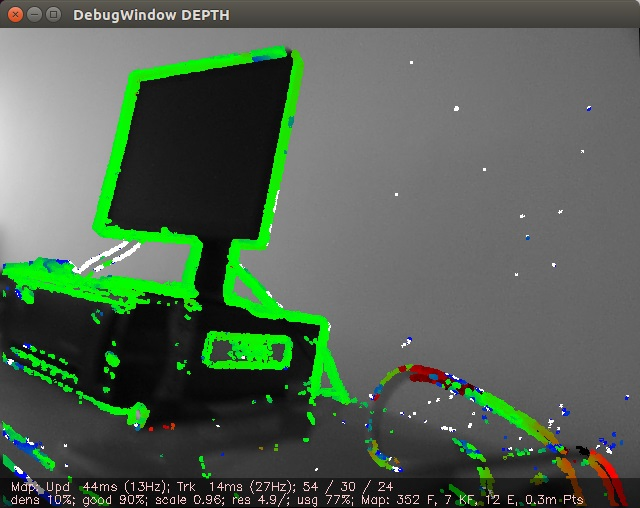
\includegraphics[width= \textwidth]{Imagens/figura3-20.jpg}
	\caption{\textit{DebugWindow DEPTH} do \texttt{live\_slam} \#1}
	\label{fig3:20}
\end{figure}

\begin{figure}[H]
	\centering
		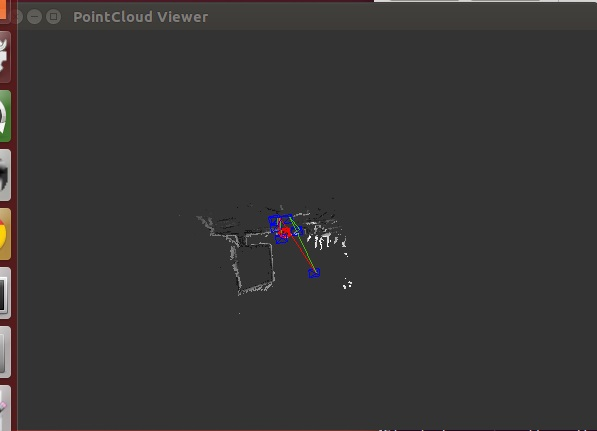
\includegraphics[width= \textwidth]{Imagens/figura3-21.jpg}
	\caption{\textit{PointCloud} referente à figura \ref{fig3:20}}
	\label{fig3:21}
\end{figure}

\begin{figure}[H]
	\centering
		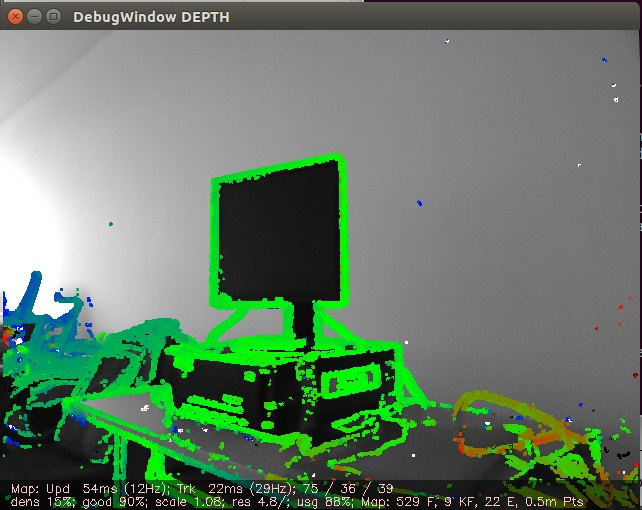
\includegraphics[width= \textwidth]{Imagens/figura3-22.jpg}
	\caption{\textit{DebugWindow DEPTH} do\texttt{ live\_slam} \#2}
	\label{fig3:22}
\end{figure}

\begin{figure}[H]
	\centering
		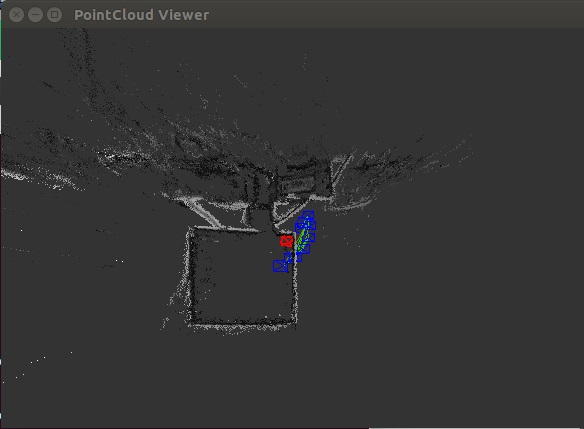
\includegraphics[width= \textwidth]{Imagens/figura3-23.jpg}
	\caption{\textit{PointCloud} referente à figura \ref{fig3:22}}
	\label{fig3:23}
\end{figure}

\begin{figure}[H]
	\centering
		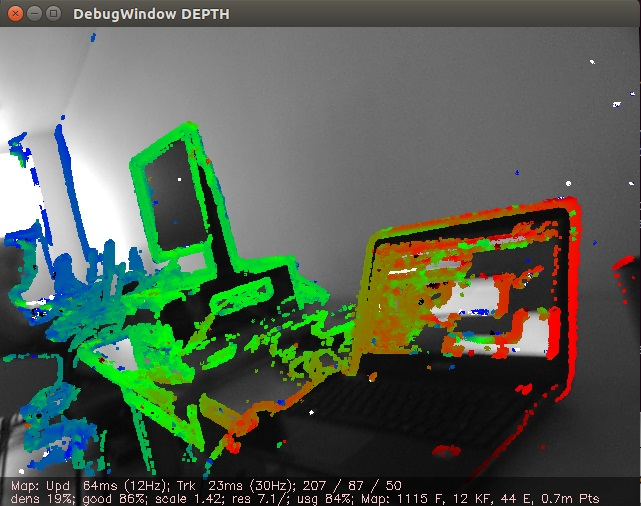
\includegraphics[width= \textwidth]{Imagens/figura3-24.jpg}
	\caption{\textit{DebugWindow DEPTH} do \texttt{live\_slam} \#3}
	\label{fig3:24}
\end{figure}

\begin{figure}[H]
	\centering
		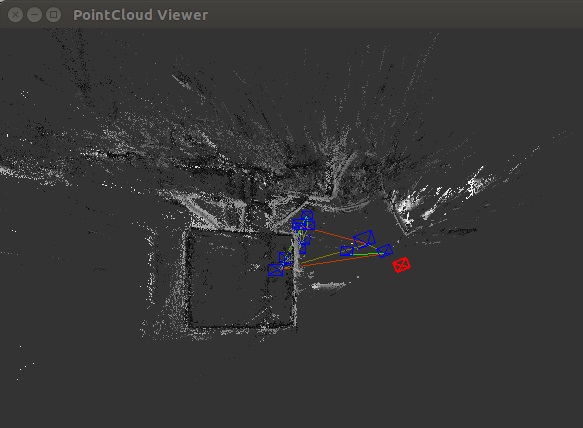
\includegraphics[width= \textwidth]{Imagens/figura3-25.jpg}
	\caption{\textit{PointCloud} referente à figura \ref{fig3:24}}
	\label{fig3:25}
\end{figure}

A saída do \texttt{lsd\_slam\_core} está sendo transferida para o visualizador na janela \textit{PointCloud Viewer} no formato de nuvem de pontos que podem ser rotacionados e observados em qualquer ângulo. A janela \textit{DebugWindow DEPTH} é a janela que oferece informações sobre a execução do algoritmo incluindo:

\begin{description}
	\item[Map upd :]{A taxa em que os quadros estão sendo computados.}
	\item[Trk :]{A taxa de quadros do \textit{dataset}/câmera.}
	\item[X/Y/Z :]{O terceiro parâmetro não possui identificação mas se encontra no formato X/Y/Z e significa rotação do quadro atual com o quadro original nos 3 eixos.}
	\item[Dens X\% :]{A densidade média dos pontos.}
	\item[Good X\% :]{ A quantidade de pontos pontos bons que podem ser utilizados pelo algoritmo, importante para verificar condições de distorção na imagem da câmera como: iluminação, foco, movimentação, taxa de bits insuficiente na compressão ou similaridade daquele quadro atual com os feitos anteriormente.}
	\item[Scale X\% :]{Escala entre os pontos.}
	\item{Número de pontos utilizados pelo algoritmo.}
	\item{Quadro atual.}
	\item{Numeração de quadro refinador por \textit{keyframe}.}
\end{description}

Além disso as cores representam o grau de proximidade de cada ponto à câmera. Pontos vermelhos são os mais próximos, pontos verdes estão à meia distância e pontos azuis são os mais distantes. Em contrapartida quanto mais azul estiver o gradiente mais longe da camera em relação ao gradiente verde está da câmera. Pontos e gradientes brancos foram reconhecidos pelo detecção de gradiente mas não conseguiu ser reconhecido em escala considerando o \textit{keyframe} atual, normalmente isso ocorre quando há uma diferença de escala inesperada como um objeto que se move ou se a iluminação ou foco da câmera atrapalhar no reconhecimento.

Essas informações são comuns tanto ao \texttt{live\_slam} quanto ao \texttt{dataset\_slam}. O método \texttt{live\_slam} se caracteriza por servir de teste do ambiente para se fazer o \textit{dataset}. Ele possui suas vantagens e desvantagens:

Vantagens:

\begin{itemize}
	\item{O funcionamento do algoritmo pode ser visto em tempo real.}
	\item{A condição de iluminação pode ser testada usando esse modo mais rapidamente.}
\end{itemize}

Desvantagens:

\begin{itemize}
	\item{É necessário utilizar em um computador portátil para que se possa mover com a câmera.}
	\item{A mobilidade enquanto se usa esse método é prejudicada.}
	\item{É mais difícil mudar os parâmetros enquanto roda o algoritmo.}
	\item{Baixa reproducibilidade.}
	\item{Alto consumo de recursos do computador.}
\end{itemize}	

Também é possível salvar o vídeo capturado usando o parâmetro do \texttt{lsd\_slam\_viewer} \textit{saveAllVideo}, no entanto essa operação é ainda mais custosa. Nas máquinas usadas para os testes, não foi possível usar essa opção.

\subsection{Obtendo o mapa 3D usando o \texttt{dataset\_slam}}

Para obter o mapa utilizando um \textit{dataset}, execute o seguinte comando:

\begin{table}[H]\label{tb:16}
\begin{tabular}{| p{\textwidth}|}
\hline
\texttt{rosrun lsd\_slam\_core dataset\_slam \_files:=/caminho/para/seu/dataset \_hz:=<hz> \_calib:=/caminho/para/seu/arquivodeccalibracao}\\
\hline
\end{tabular}
\caption{Comando para executar o \texttt{dataset\_slam} com um arquivo de calibração externo}
\end{table}

Troque \texttt{/caminho/para/seu/dataset} pelo caminho do seu \textit{dataset}, \texttt{<hz>} idealmente deverá ser trocado para 0, o que permite o rastreamento e mapeamento sequencial, mas haverá uma queda de desempenho do que a contrapartida em tempo real. Por fim, troque \texttt{/caminho/para}\\ \texttt{/seu/arquivodeccalibracao} pelo caminho do seu arquivo de configuração resultante na seção 3.2.3.6. Segue abaixo algumas capturas de tela com o comando sendo executado:

\begin{figure}[H]
	\centering
		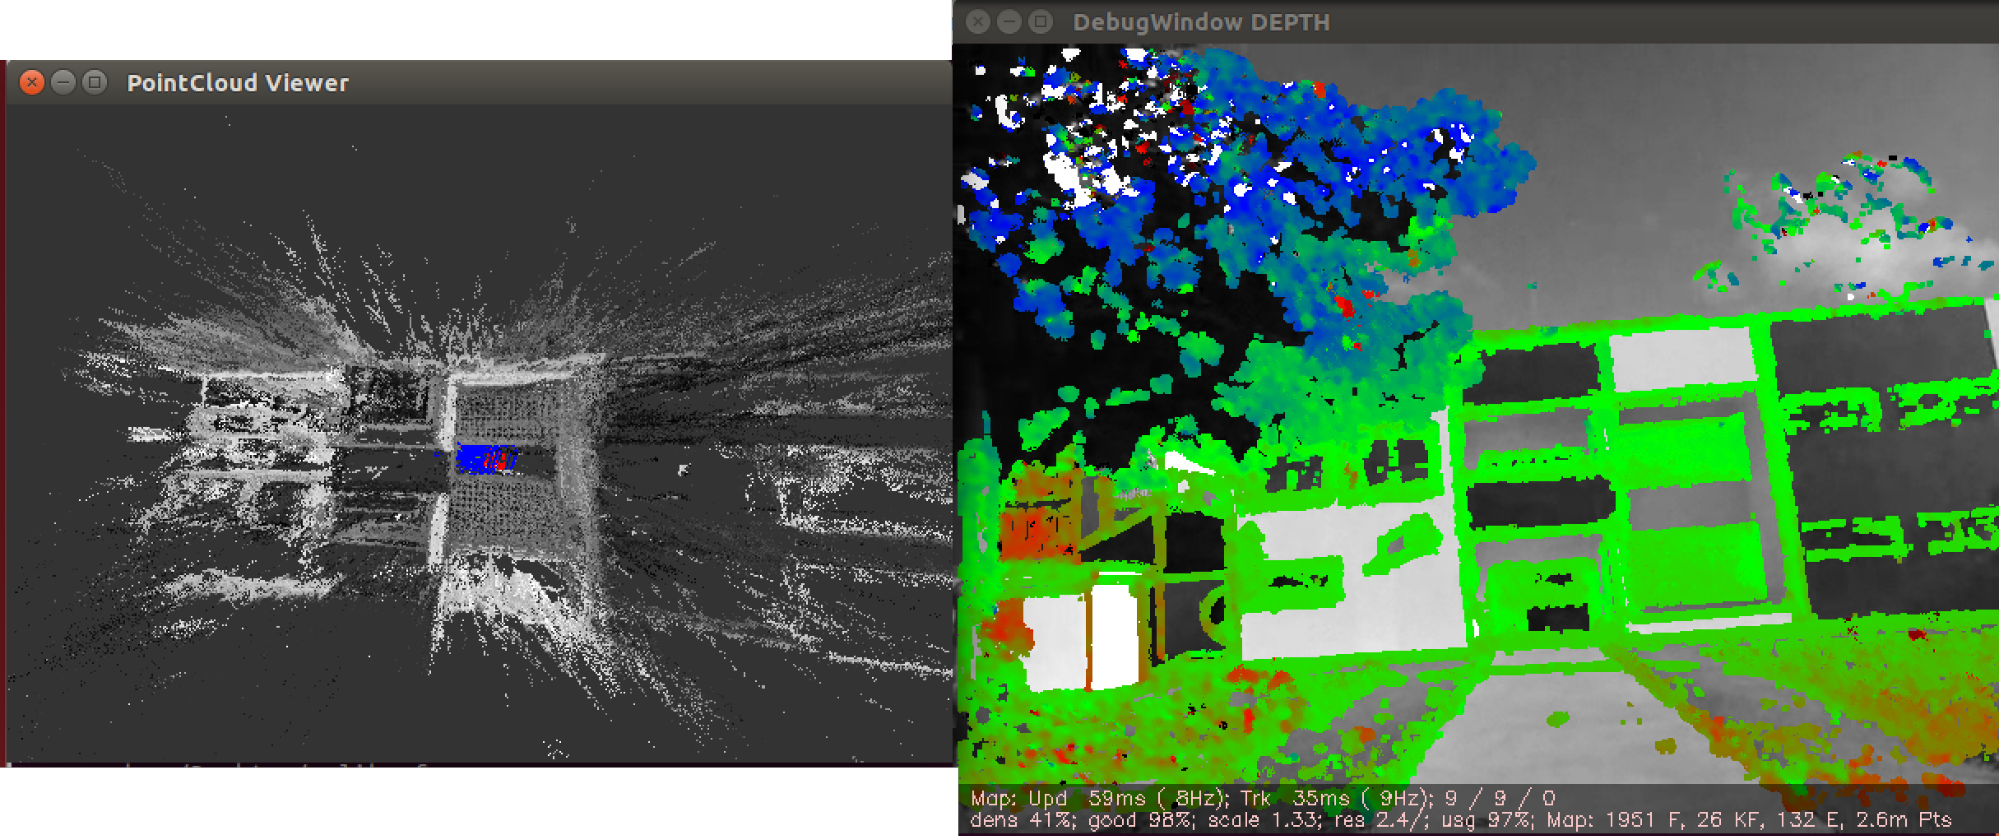
\includegraphics[width= \textwidth]{Imagens/figura3-26E3-27.png}
	\caption{\textit{PointCloud} e \textit{DebugWindow DEPTH} do \texttt{dataset\_slam} \#1}
	\label{fig3:26}
\end{figure}





\begin{figure}[H]
	\centering
		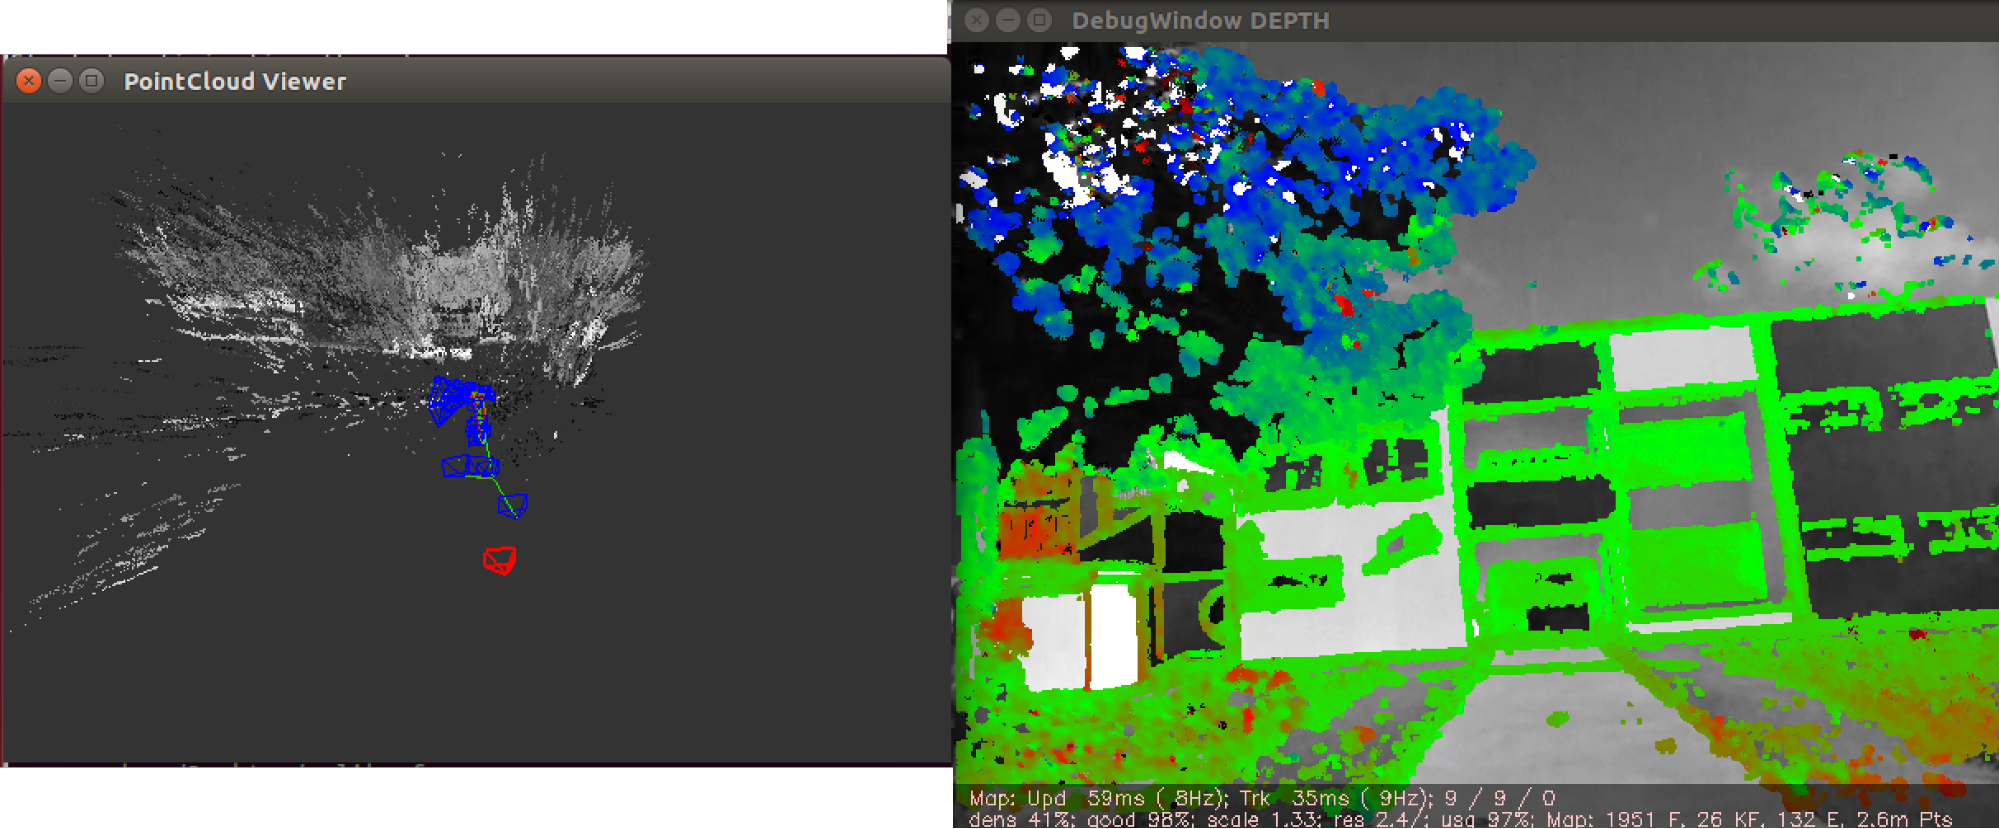
\includegraphics[width= \textwidth]{Imagens/figura3-28E3-29.png}
	\caption{\textit{PointCloud} e \textit{DebugWindow DEPTH} do \texttt{dataset\_slam} \#4}
	\label{fig3:27}
\end{figure}

É necessário também, dependendo do \textit{dataset} usado, um refinamento dos parâmetros de visualização e também da forma que o \texttt{lsd\_slam\_core} opera, pois com os parâmetros padrão é possível perceber que a grama em frente ao prédio atrapalhou a captura dos gradientes.

\subsection{Parâmetros \texttt{rqt\_reconfigure}}

Uma característica fundamental da ferramenta é a capacidade de modificar alguns parâmetros do algoritmo, esses parâmetros podem ser modificados usando a ferramenta \texttt{rqt\_reconfigure} que vem junto com o pacote do \textit{LSD-SLAM} que pode ser chamado usando o seguinte comando:

\begin{table}[H]\label{tb:17}
\begin{tabular}{| p{\textwidth}|}
\hline
\texttt{rosrun rqt\_reconfigure rqt\_reconfigure}\\
\hline
\end{tabular}
\caption{Comando para inicialização do \texttt{rqt\_reconfigure}}
\end{table}

E então será aberta uma janela com vários parâmetros dependendo de quais janelas do \textit{LSD-SLAM} estão abertas, isto é, o \texttt{lsd\_slam\_core} e o \texttt{lsd\_slam\_viewer}. Para cada uma das janelas os parâmetros podem ser modificados em tempo real. A figura 3.30 mostra alguns parâmetros de configuração.

\begin{figure}[H]
	\centering
		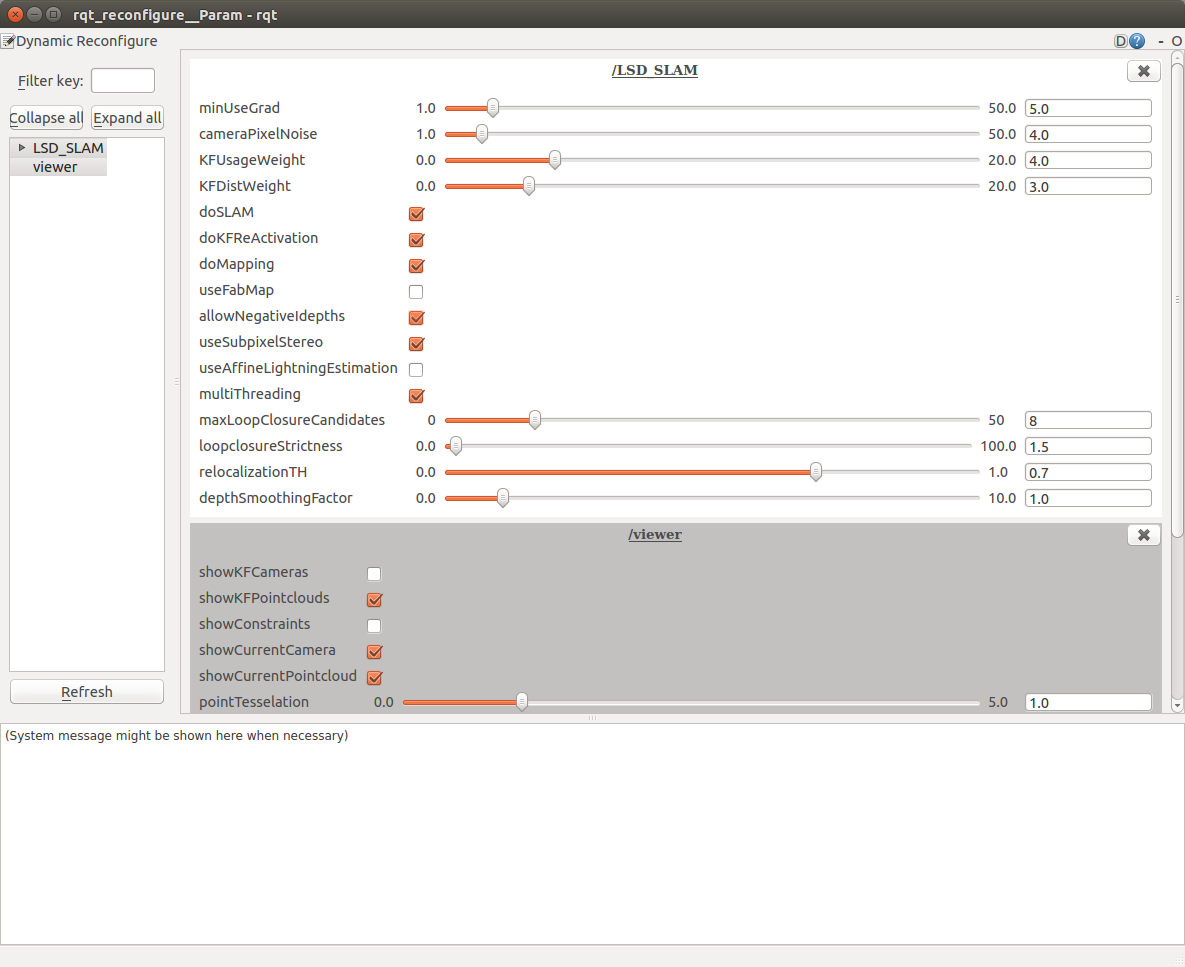
\includegraphics[width= \textwidth]{Imagens/figura3-30.png}
	\caption{Tela do \texttt{rqt\_reconfigure}}
	\label{fig3:28}
\end{figure}



\subsubsection{\textit{minUseGrad}}

Esse parâmetro indica a extensão mínima do gradiente para que o algoritmo o reconheça. Em outras palavras, quanto maior esse valor, mais restritiva será a captura de gradientes. Diminuindo esse parâmetro, gradientes pequenos como texturas irregulares, grama e outros gradientes não uniformes serão reconhecidos. Deve-se analisar cuidadosamente o quanto do ambiente deseja-se capturar e ajustar esse parâmetro de acordo, assim como o exemplo a seguir:

\begin{figure}[H]
	\centering
		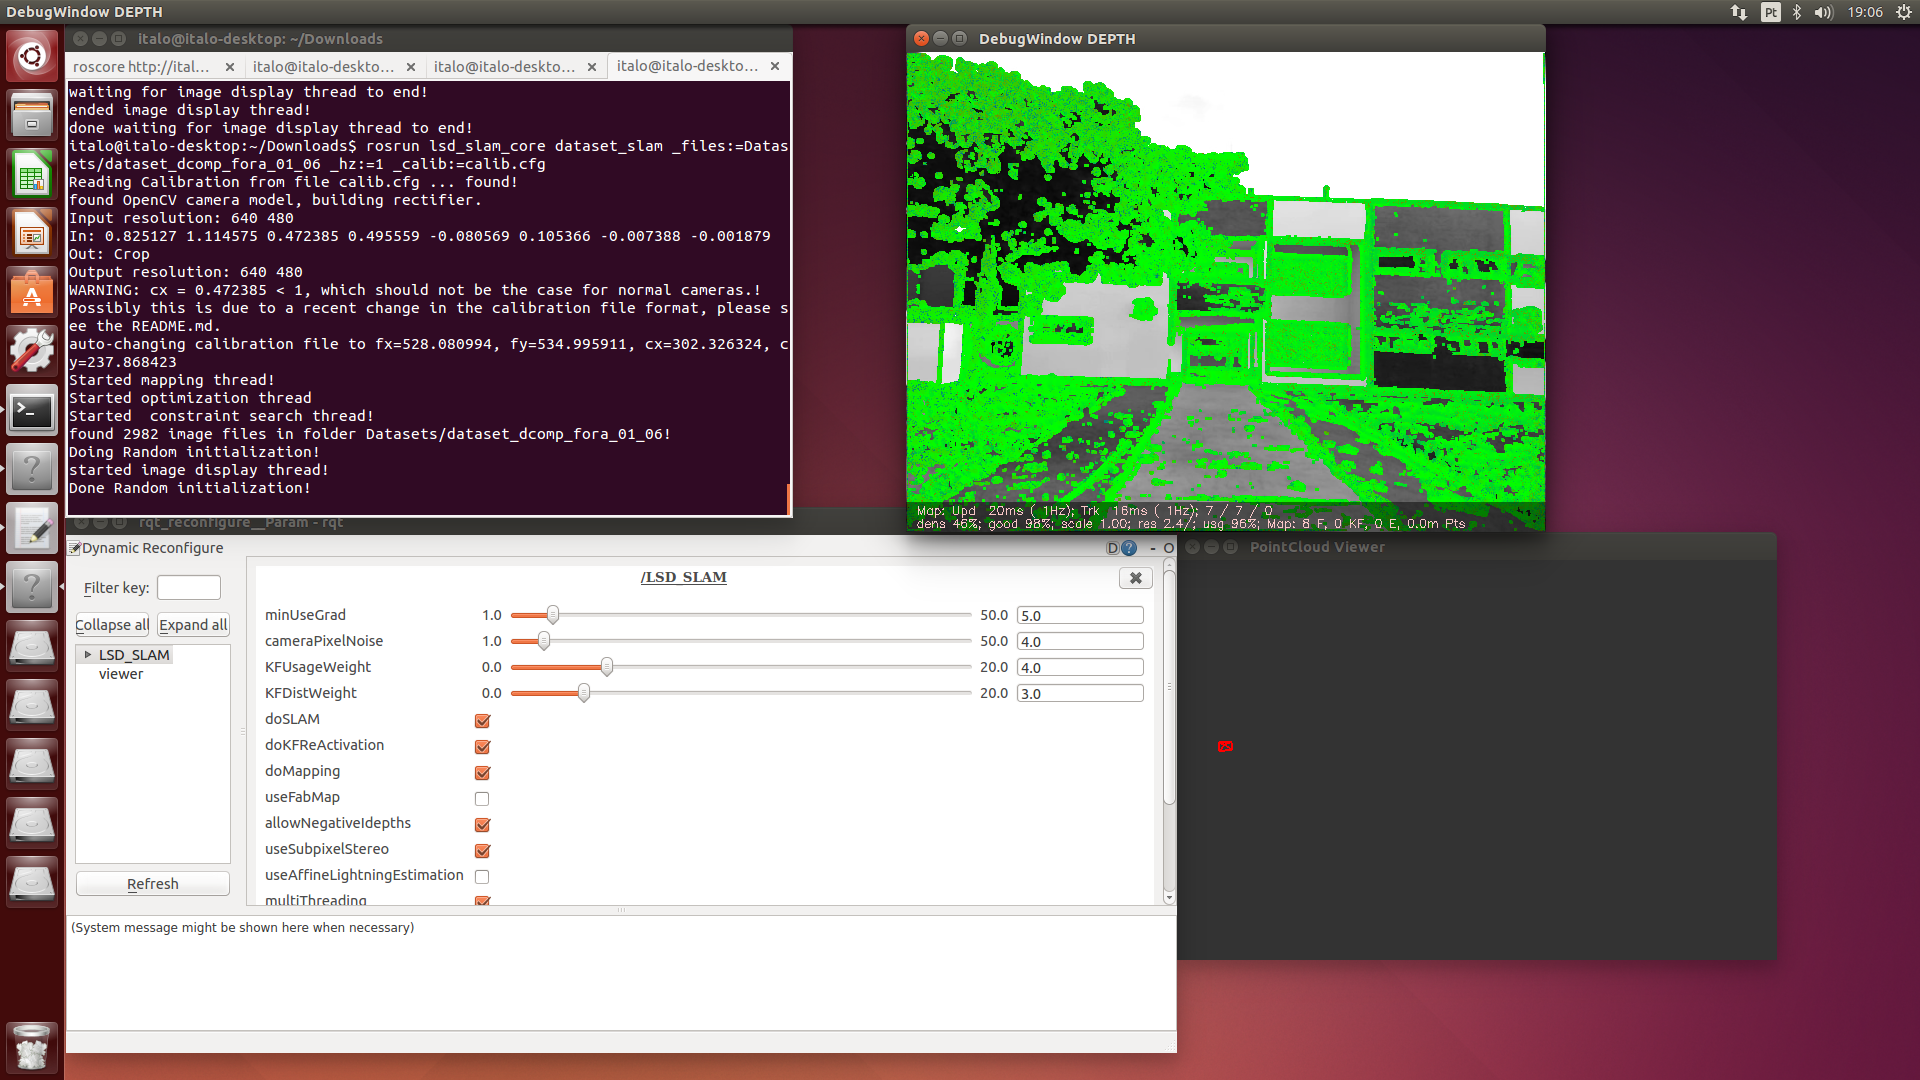
\includegraphics[width= \textwidth]{Imagens/figura3-31.png}
	\caption{\textit{minUseGrad} no seu valor padrão de 5.0}
	\label{fig3:29}
\end{figure}

\begin{figure}[H]
	\centering
		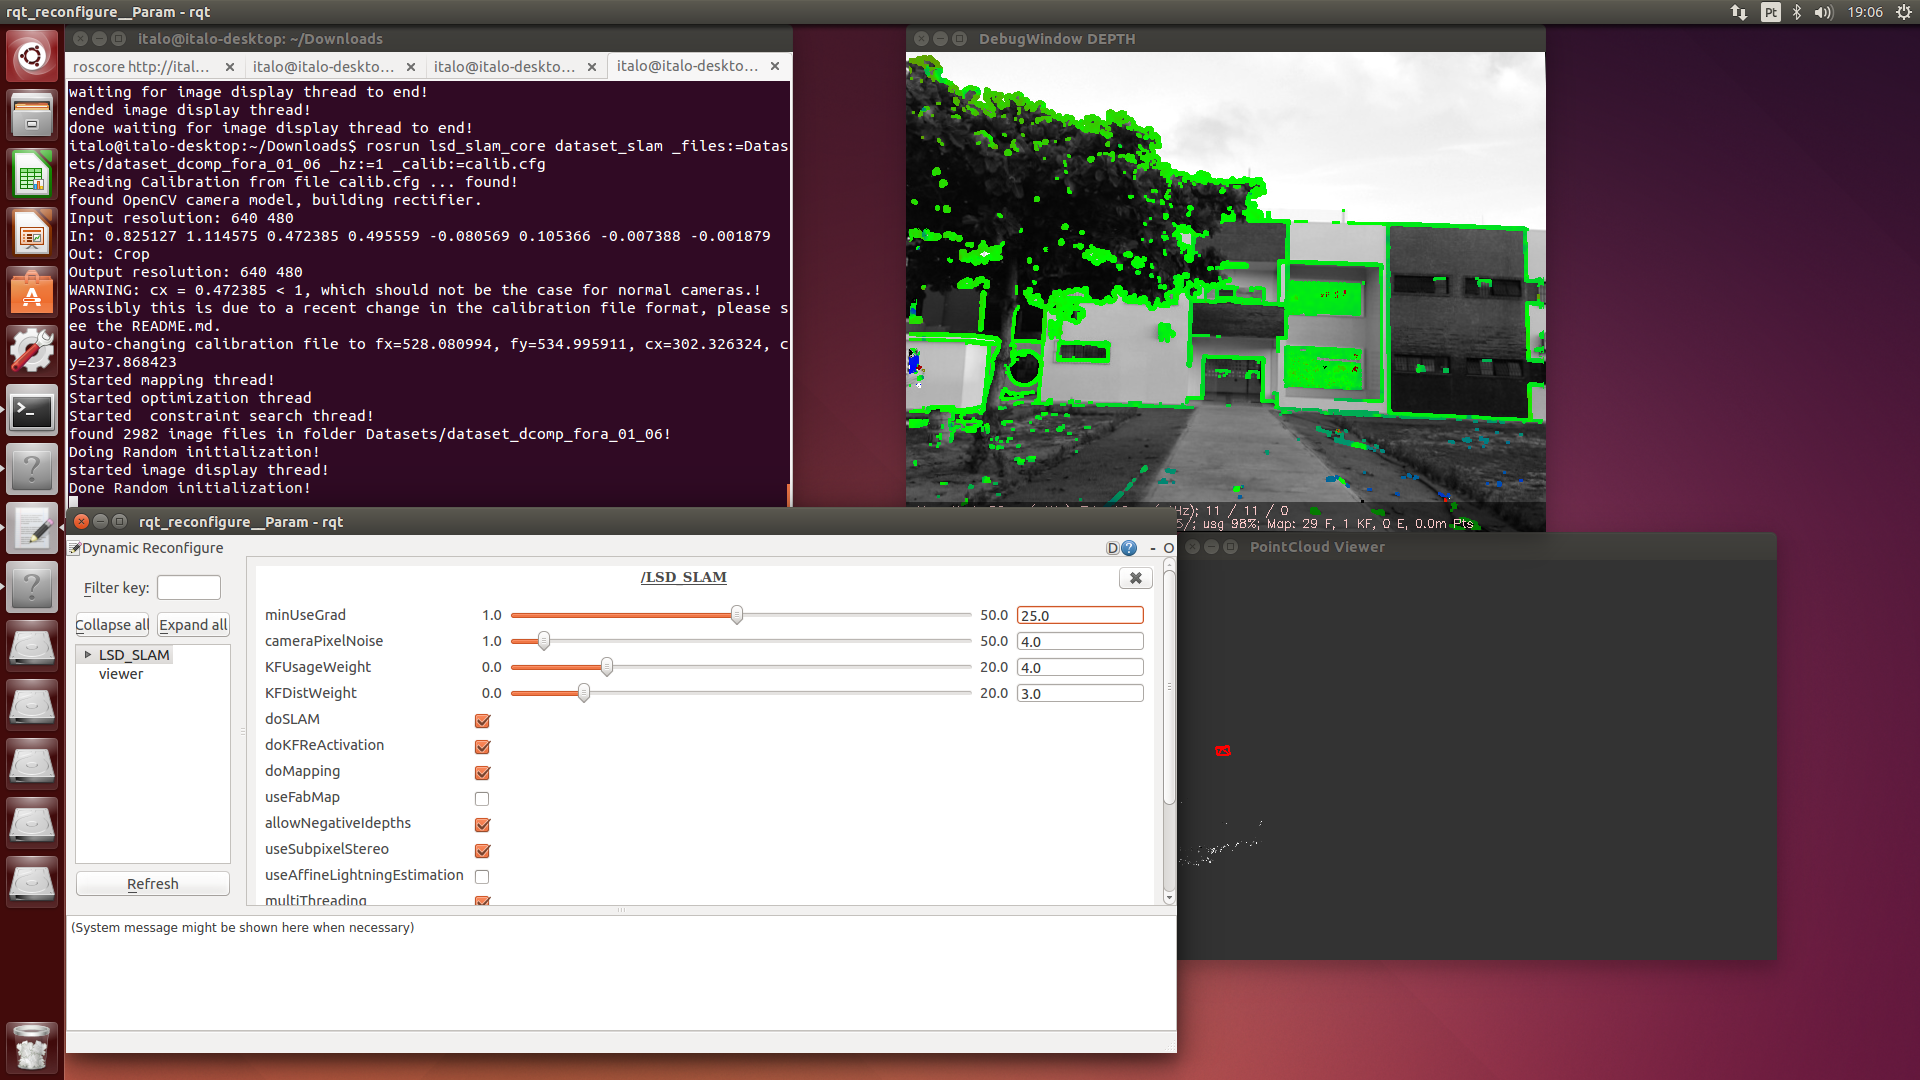
\includegraphics[width= \textwidth]{Imagens/figura3-32.png}
	\caption{\textit{minUseGrad} em 25.0}
	\label{fig3:30}
\end{figure}

Pelos exemplos pode-se perceber que usar o \textit{minUseGrad} no seu valor padrão de 5.0 acrescenta muito ruído devido à grama, além da própria grama ser uma textura que pode ser facilmente confundida gerando erros de relocalização mais à frente na execução. Ao diminuir o parâmetro, a continuidade do gradiente precisa ser mais uniforme para poder ser aceito pelo algoritmo. Não há heurística para a escolha desse valor e ele deve ser testado para cada ambiente. Também vale frisar que aumentar demais esse valor pode cortar alguns gradientes perfeitamente utilizáveis mas que são menos uniformes como por exemplo a passarela até o prédio na imagem.

\subsubsection{\textit{KFUsageWeight e KFDistanceWeight}}


Esses parâmetros influenciam na frequência em que novos \textit{keyframes} são obtidos. O \textit{KFUsageWeight} é em razão da quantidade de quadros usados para refinar, de forma que um número maior faz com que o algoritmo capture novos \textit{keyframes} diminuindo a quantidade de refinamento em cada um consequentemente, como no exemplo a seguir:

\begin{figure}[H]
	\centering
		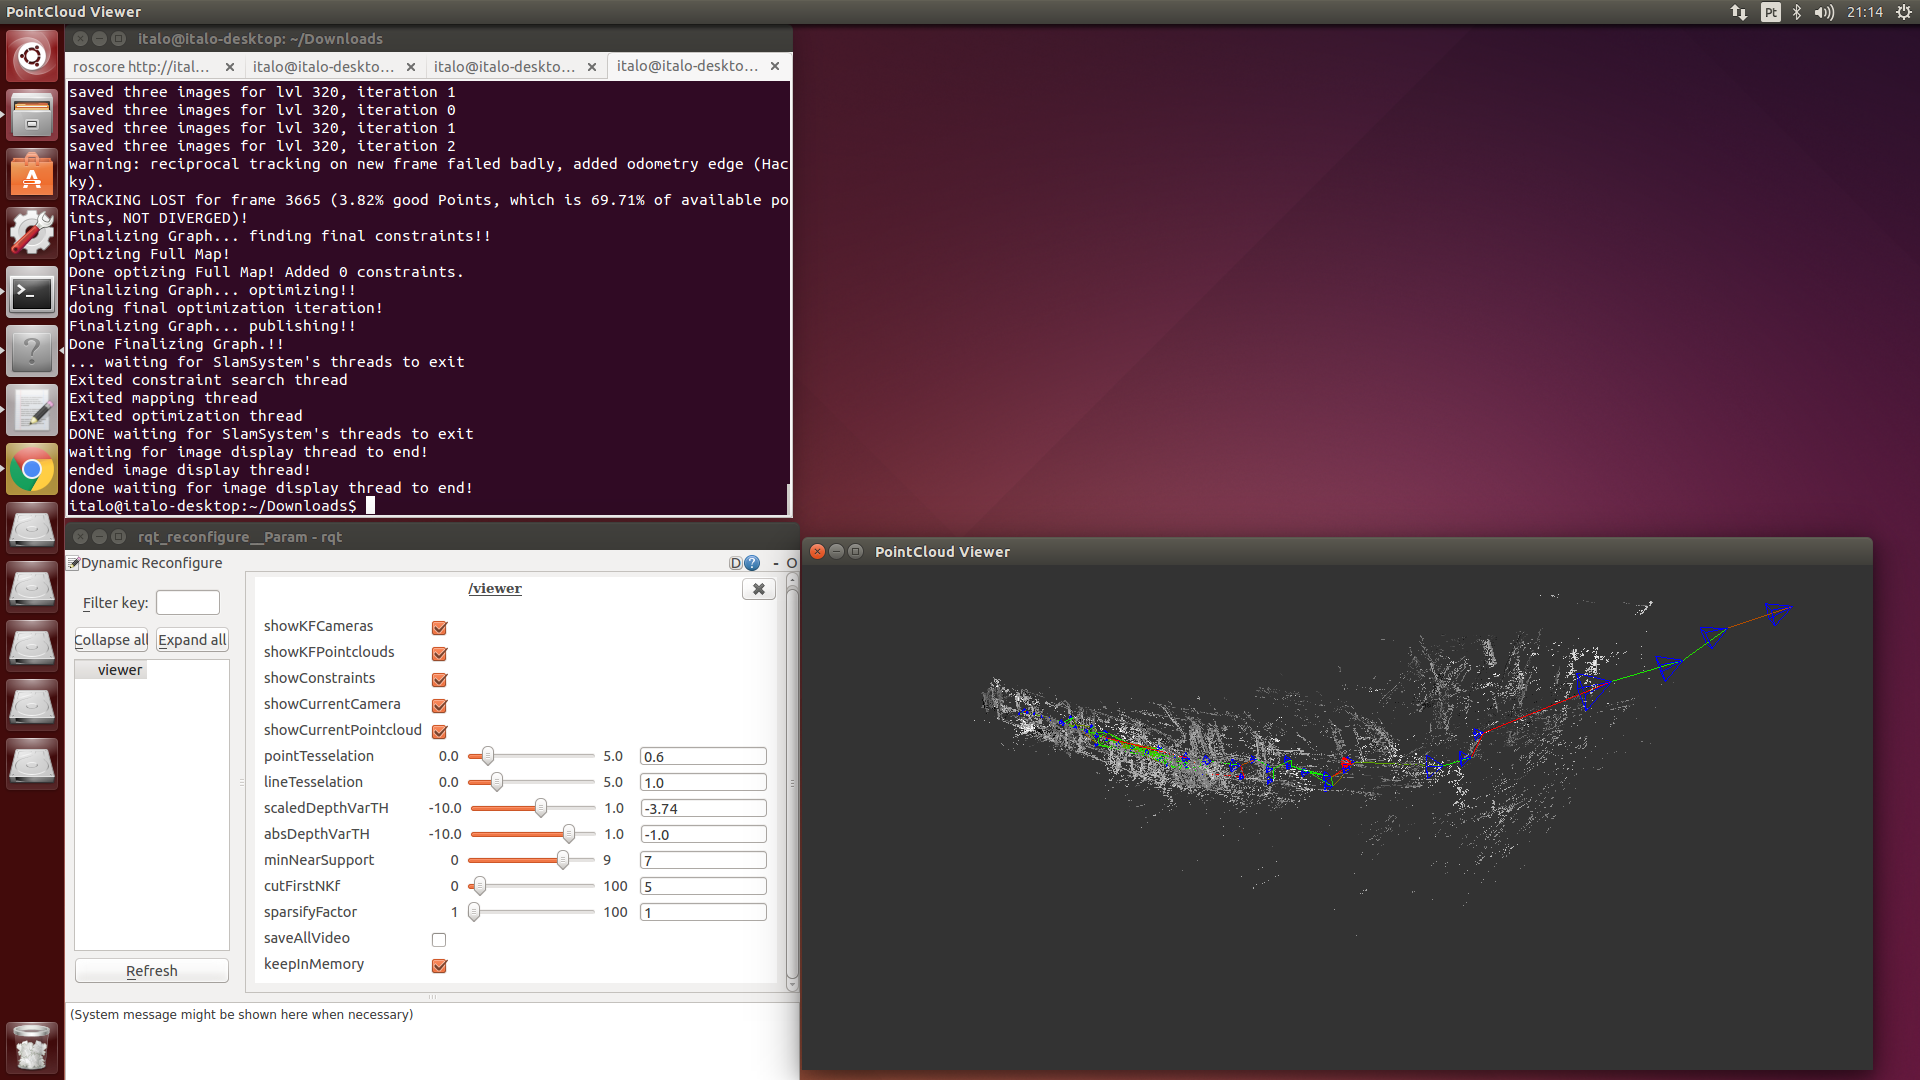
\includegraphics[width= \textwidth]{Imagens/figura3-33.png}
	\caption{\textit{PointCloud} e \textit{keyframes} do corredor do 1º andar do DCOMP usando o \textit{KFUsageWeight} padrão de 4.0 e \textit{KFDistWeight} padrão de 3.0}
	\label{fig3:31}
\end{figure}

\begin{figure}[H]
	\centering
		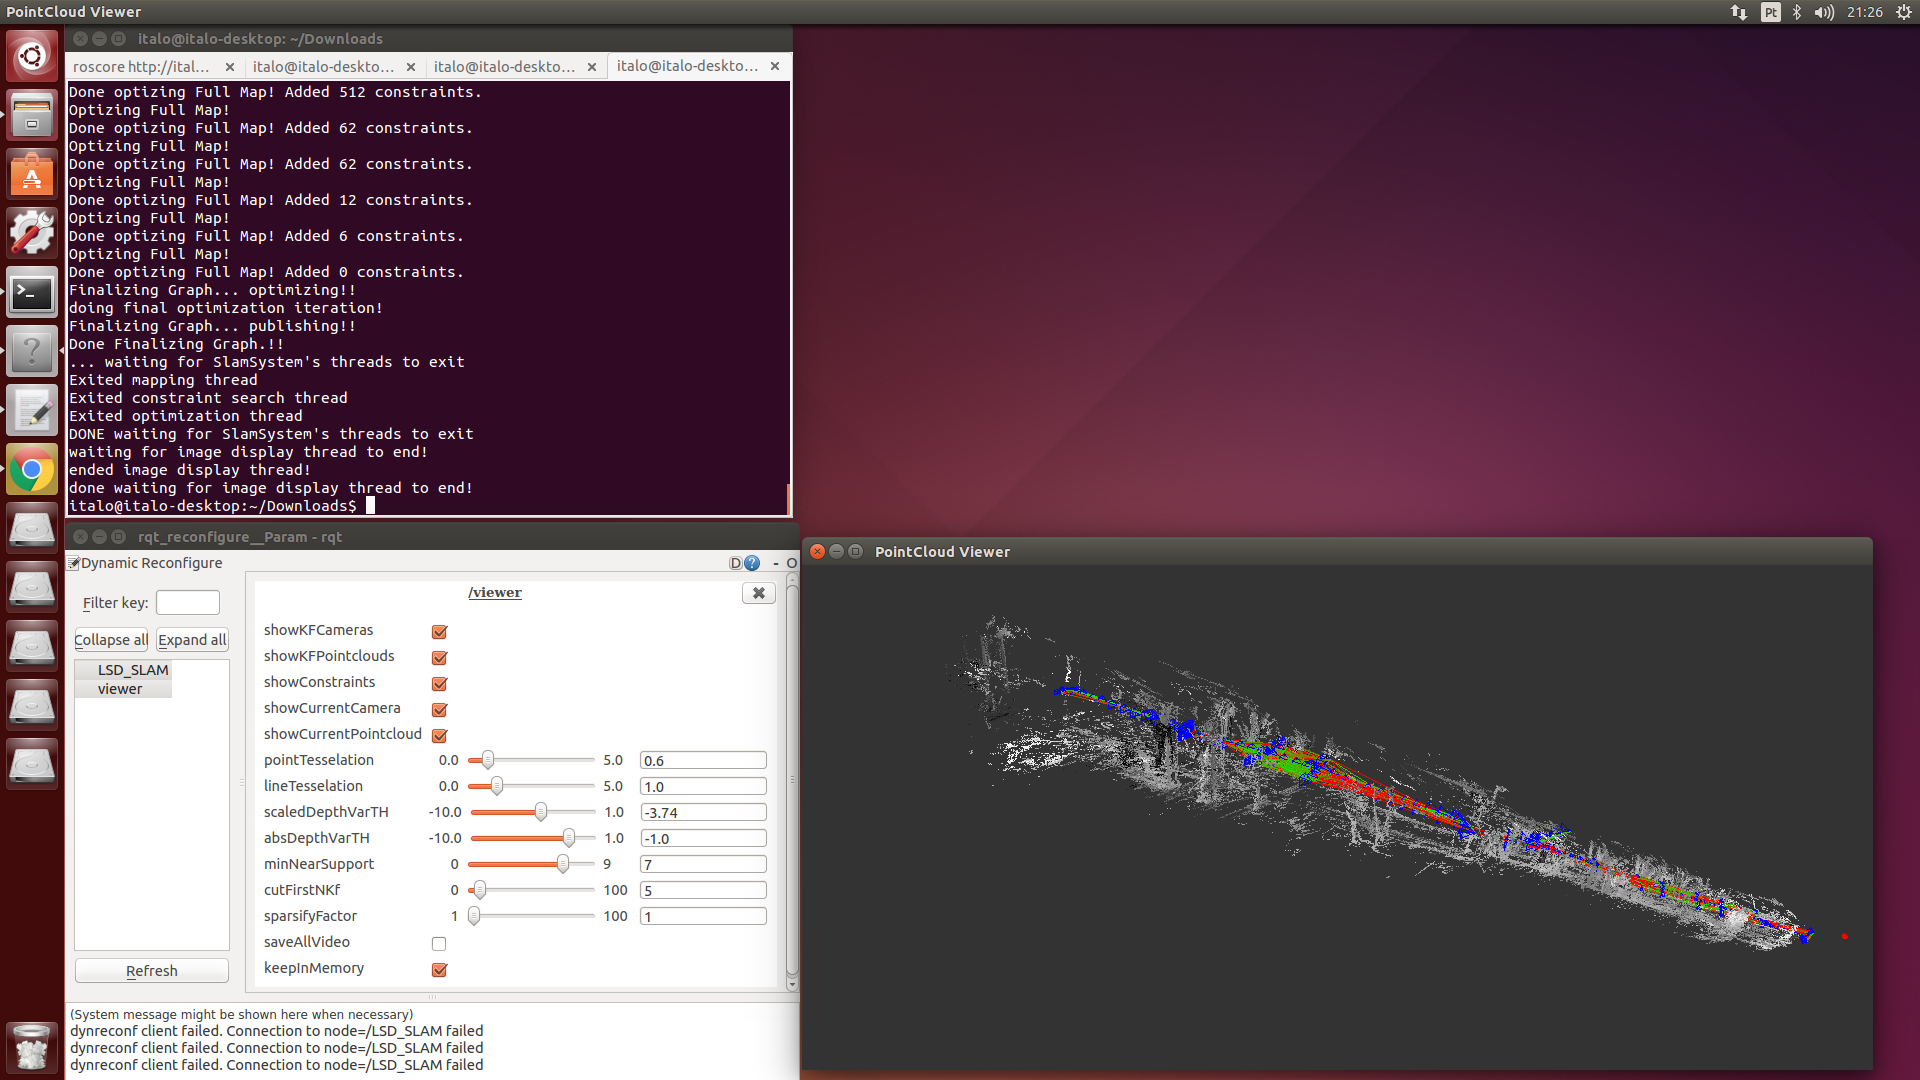
\includegraphics[width= \textwidth]{Imagens/figura3-34.png}
	\caption{\textit{PointCloud} e \textit{keyframes} do corredor do 1º andar do DCOMP usando o \textit{KFUsageWeight} máximo de 20.0 \#1}
	\label{fig3:32}
\end{figure}

\begin{figure}[H]
	\centering
		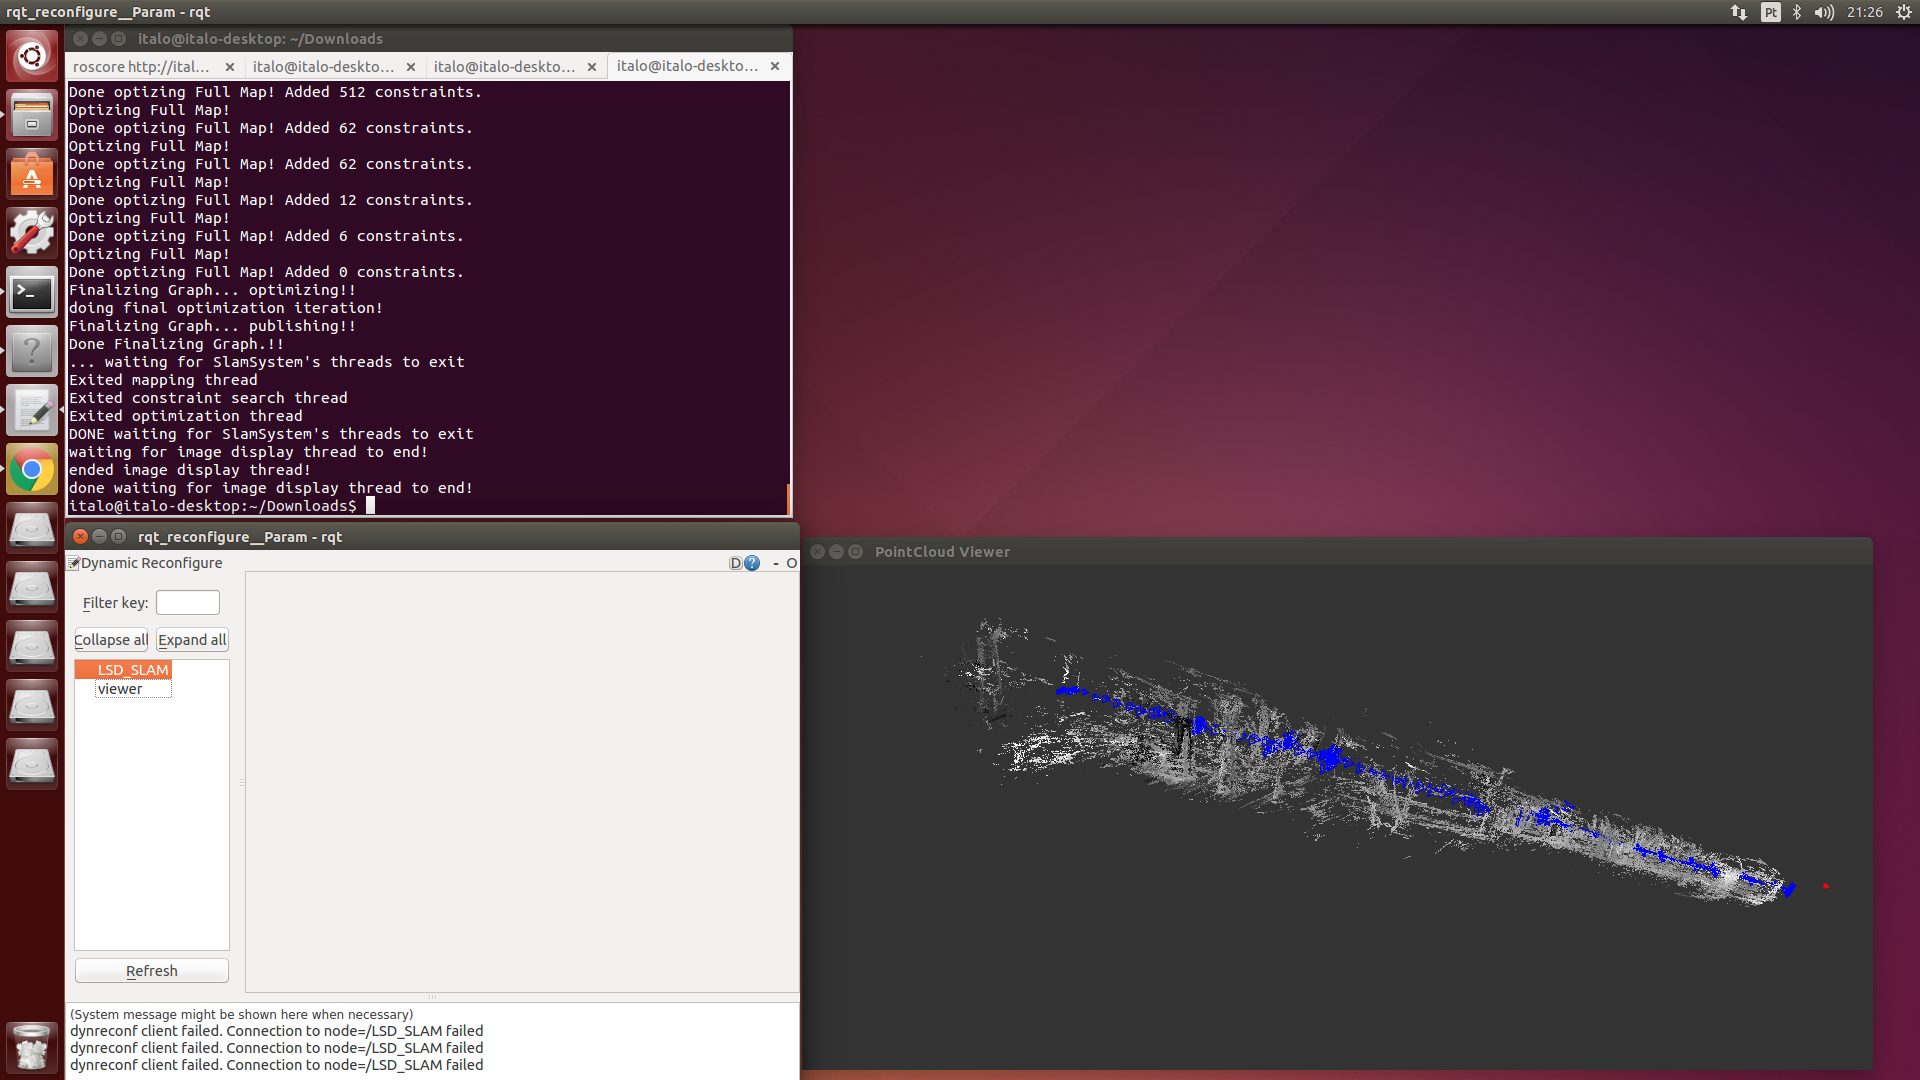
\includegraphics[width= \textwidth]{Imagens/figura3-35}
	\caption{\textit{PointCloud} e \textit{keyframes} do corredor do 1º andar do DCOMP usando o \textit{KFUsageWeight} máximo de 20.0 \#2}
	\label{fig3:33}
\end{figure}


\begin{figure}[H]
	\centering
		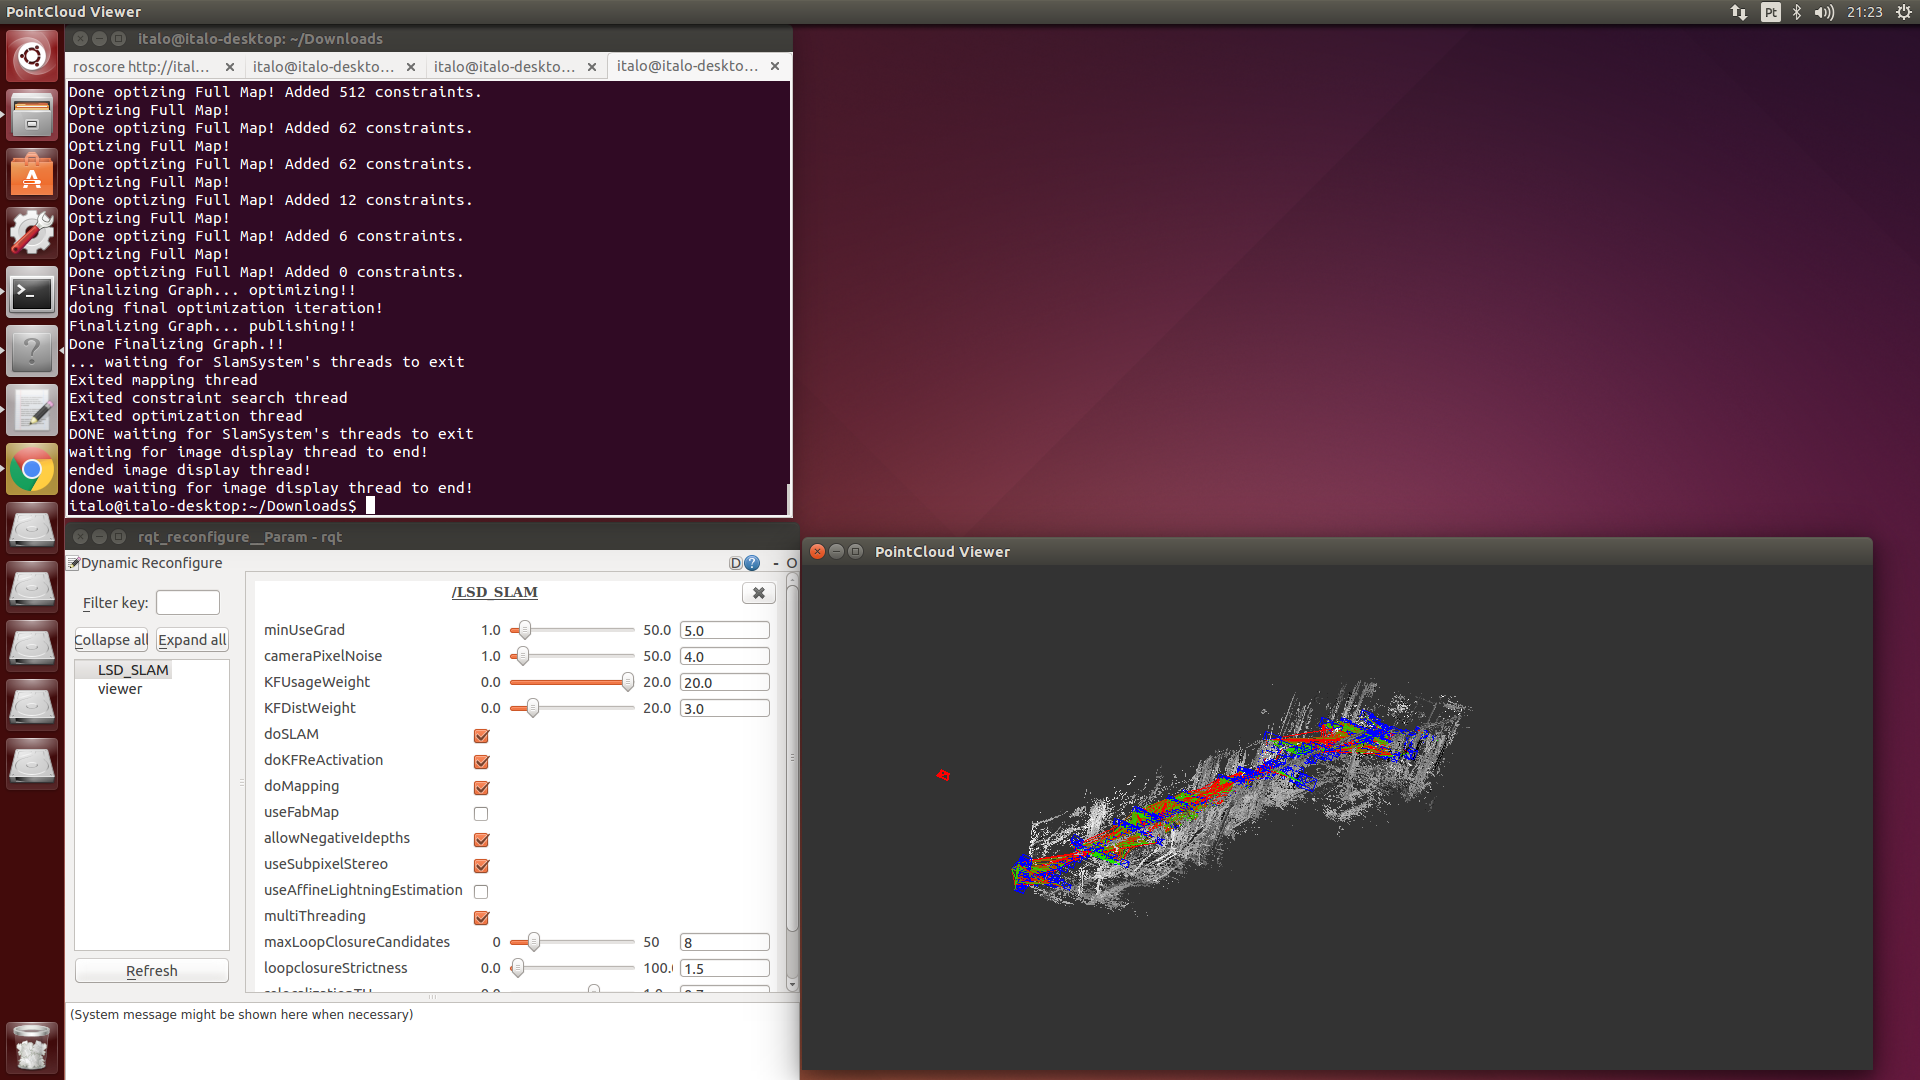
\includegraphics[width= \textwidth]{Imagens/figura3-36.png}
	\caption{\textit{PointCloud} e \textit{keyframes} do corredor do 1º andar do DCOMP usando o \textit{KFUsageWeight} máximo de 20.0 \#3}
	\label{fig3:34}
\end{figure}


\begin{figure}[H]
	\centering
		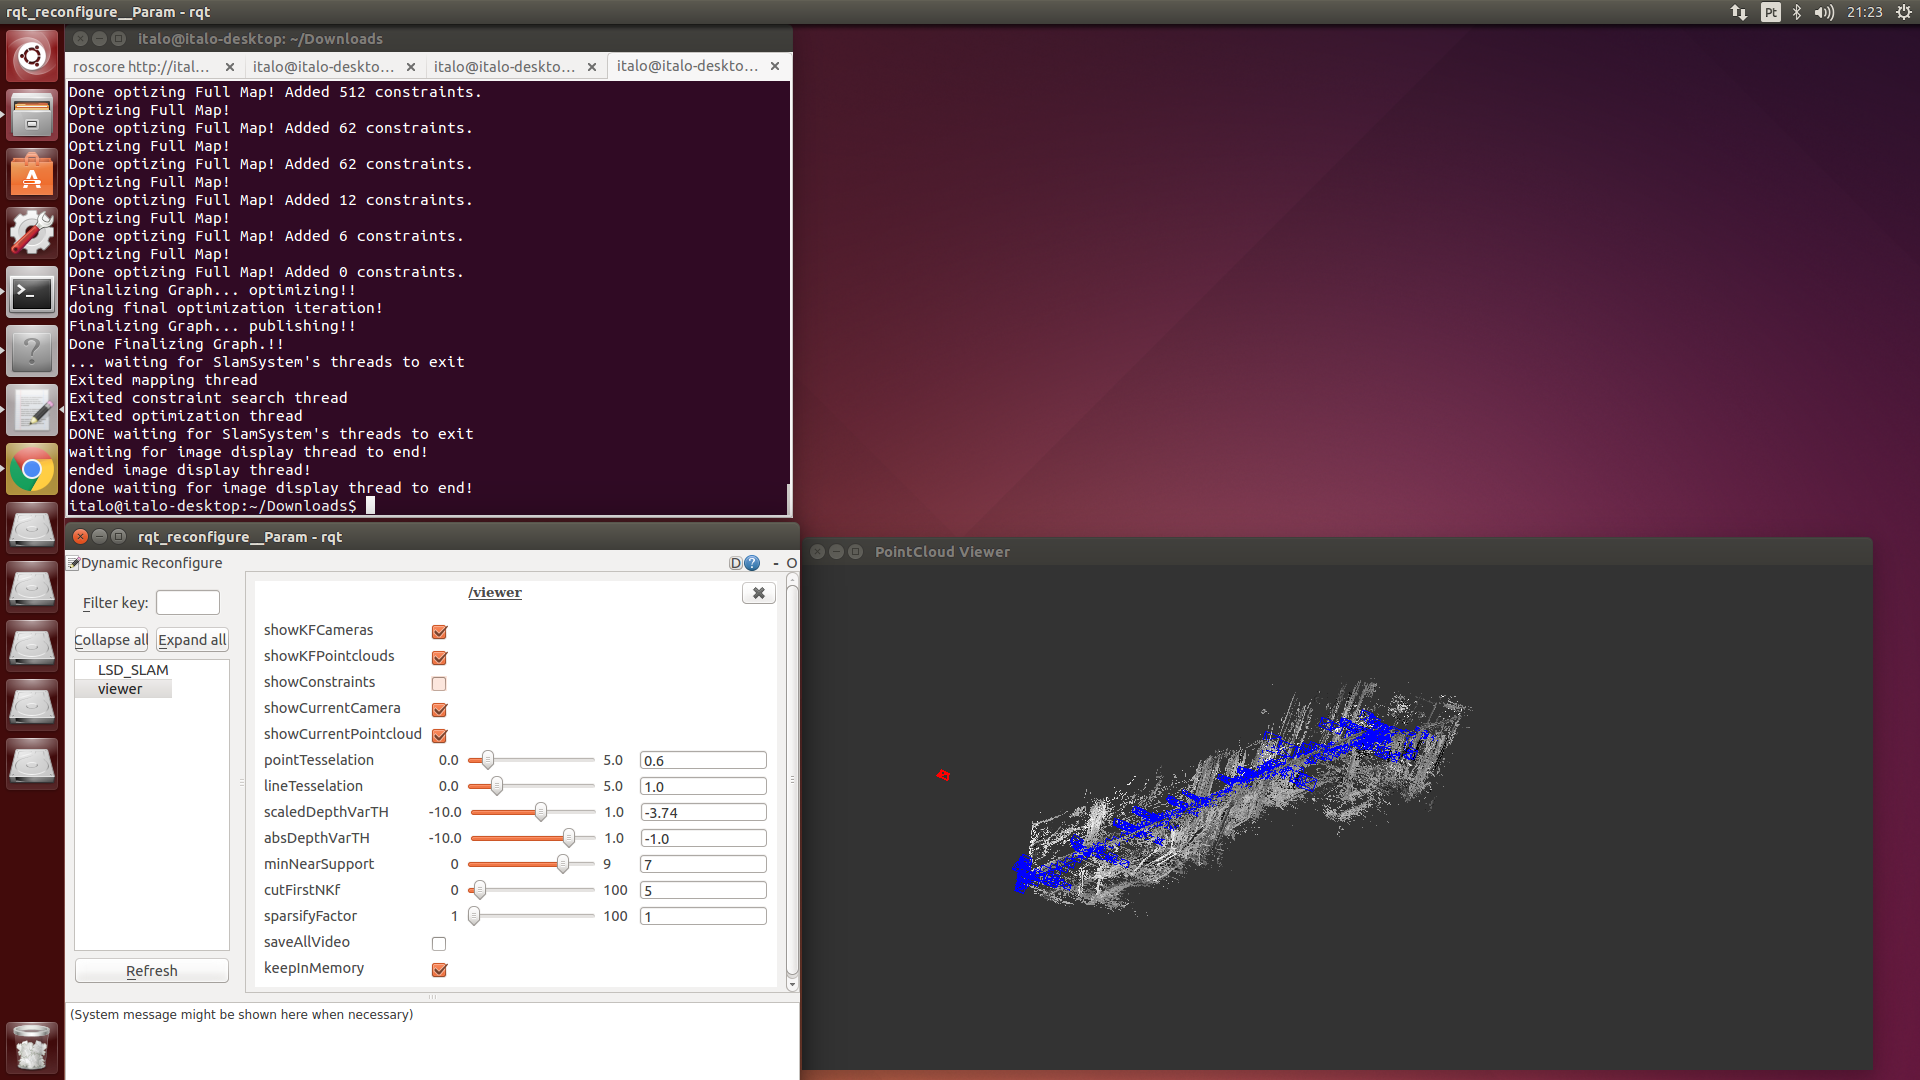
\includegraphics[width= \textwidth]{Imagens/figura3-37.png}
	\caption{\textit{PointCloud} e \textit{keyframes} do corredor do 1º andar do DCOMP usando o \textit{KFUsageWeight} máximo de 20.0 \#4}
	\label{fig3:35}
\end{figure}


Nas janelas do \textit{PointCloud}, as linhas verdes e vermelhas representam \textit{constraints} entre \textit{keyframes} e as pirâmides azuis são \textit{keyframes} e a posição da câmera em relação ao modelo total. Percebe-se que o valor padrão não reproduziu um resultado tão bom quanto o valor máximo, e também pode-se ver que há muito mais \textit{constraints} e \textit{keyframes} nas imagem com o valor máximo. Mas apesar de se ter obtido um resultado melhor dessa forma, há uma carga muito maior de processamento do que pelo valor padrão, fazendo o computador demorar muito mais para executar essa operação devido a quantidade maior de \textit{keyframes} que o algoritmo tem que rastrear e interligar, a ponto dela não ser bem aplicada no \texttt{live\_slam}, e nem em computadores mais lentos/com menor capacidade de processamento. Da mesma forma o \textit{KFDistWeight} também modifica a quantidade de \textit{keyframes}, mas ao contrário do \textit{KFUsageWeight}, ele faz a partir da distância, ou seja, caso o \textit{dataset} possua vários quadros bem próximos fisicamente um do outro e outros quadros mais afastados poderá haver diminuição de \textit{keyframes} no primeiro caso e o aumento de \textit{keyframes} no segundo caso. Isso faz com que o refinamento dos \textit{keyframes} seja mais dependente do \textit{dataset} fazendo com que seja necessário um cuidado maior na hora de movimentar a câmera para não acabar coletando uma quantidade insuficiente de quadros naquela localização. Segue abaixo o mesmo \textit{dataset} usado acima só que com o valor máximo do \textit{KFDistWeight}.

\begin{figure}[H]
	\centering
		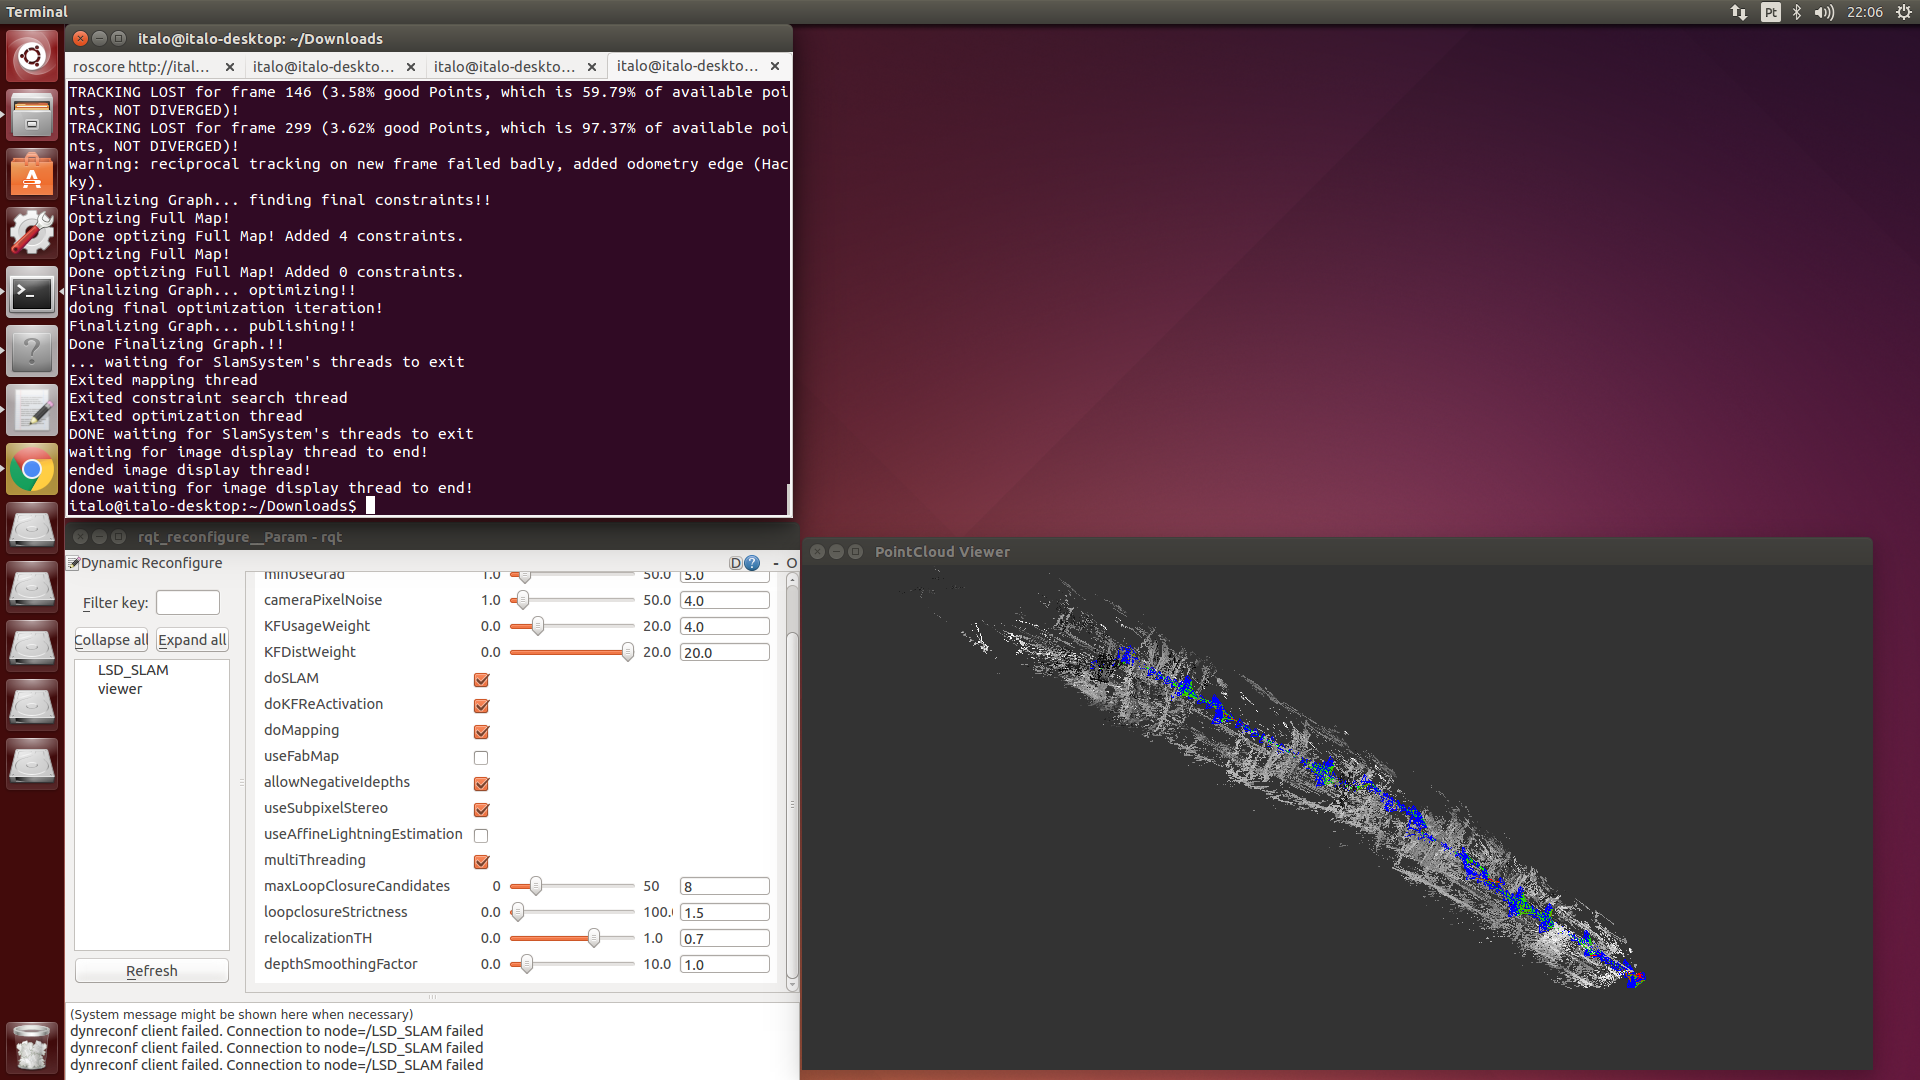
\includegraphics[width= \textwidth]{Imagens/figura3-38.png}
	\caption{\textit{PointCloud} e \textit{keyframes} do corredor do 1º andar do DCOMP usando o \textit{KFDistWeight} máximo de 20.0 \#1}
	\label{fig3:36}
\end{figure}

\begin{figure}[H]
	\centering
		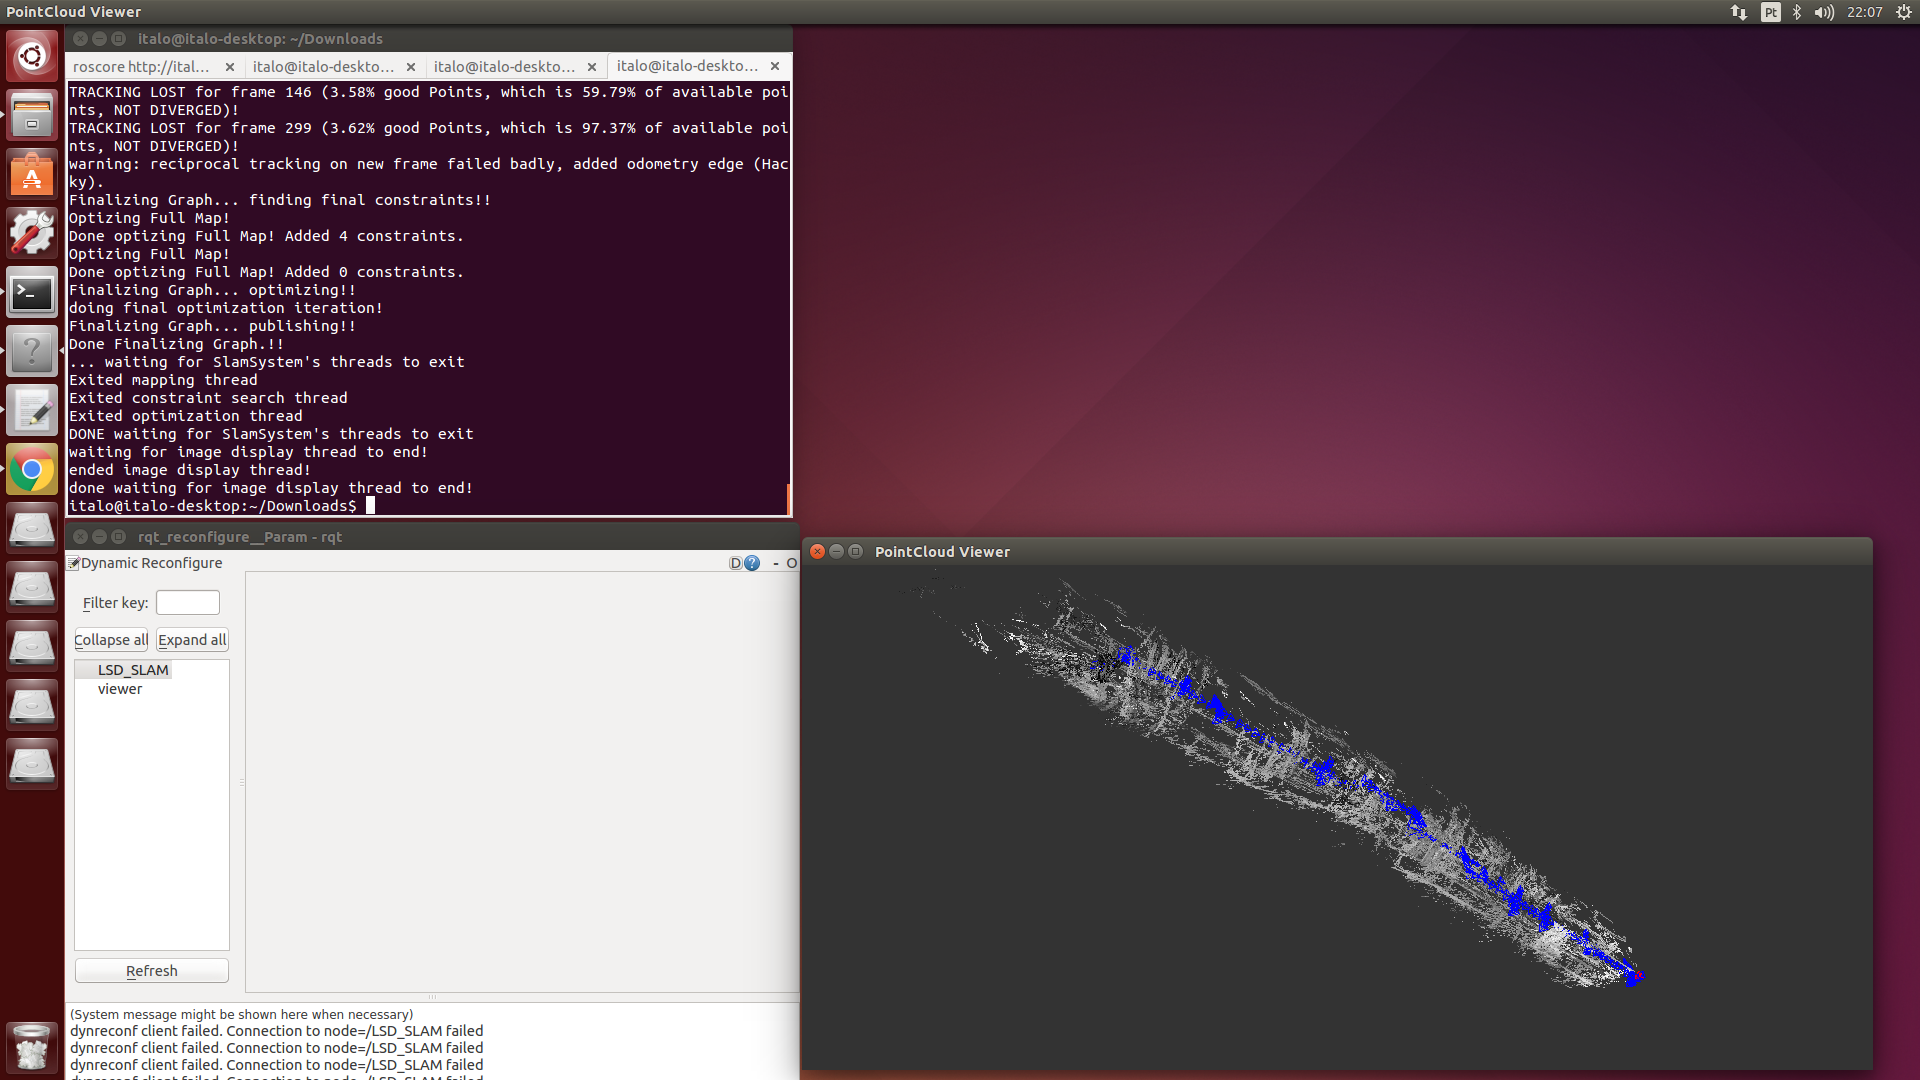
\includegraphics[width= \textwidth]{Imagens/figura3-39.png}
	\caption{\textit{PointCloud} e \textit{keyframes} do corredor do 1º andar do DCOMP usando o \textit{KFDistWeight} máximo de 20.0 \#2}
	\label{fig3:37}
\end{figure}

Como o novo exemplo demonstra, os \textit{keyframes} se comparados aos do valor padrão são mais numerosos, e o resultado geral também foi melhor. O aumento do parâmetro não é tão custoso para máquina como é no \textit{KFUsageWeight}, assim há a possibilidade de usá-lo em computadores com poder de processamento reduzido ou no \texttt{live\_slam}. É importante a experimentação desses parâmetros para se obter o melhor resultado dependendo do \textit{dataset} utilizado e a máquina utilizada. Para concluir essa seção, segue um exemplo do valor máximo de ambos os parâmetros juntos.

\begin{figure}[H]
	\centering
		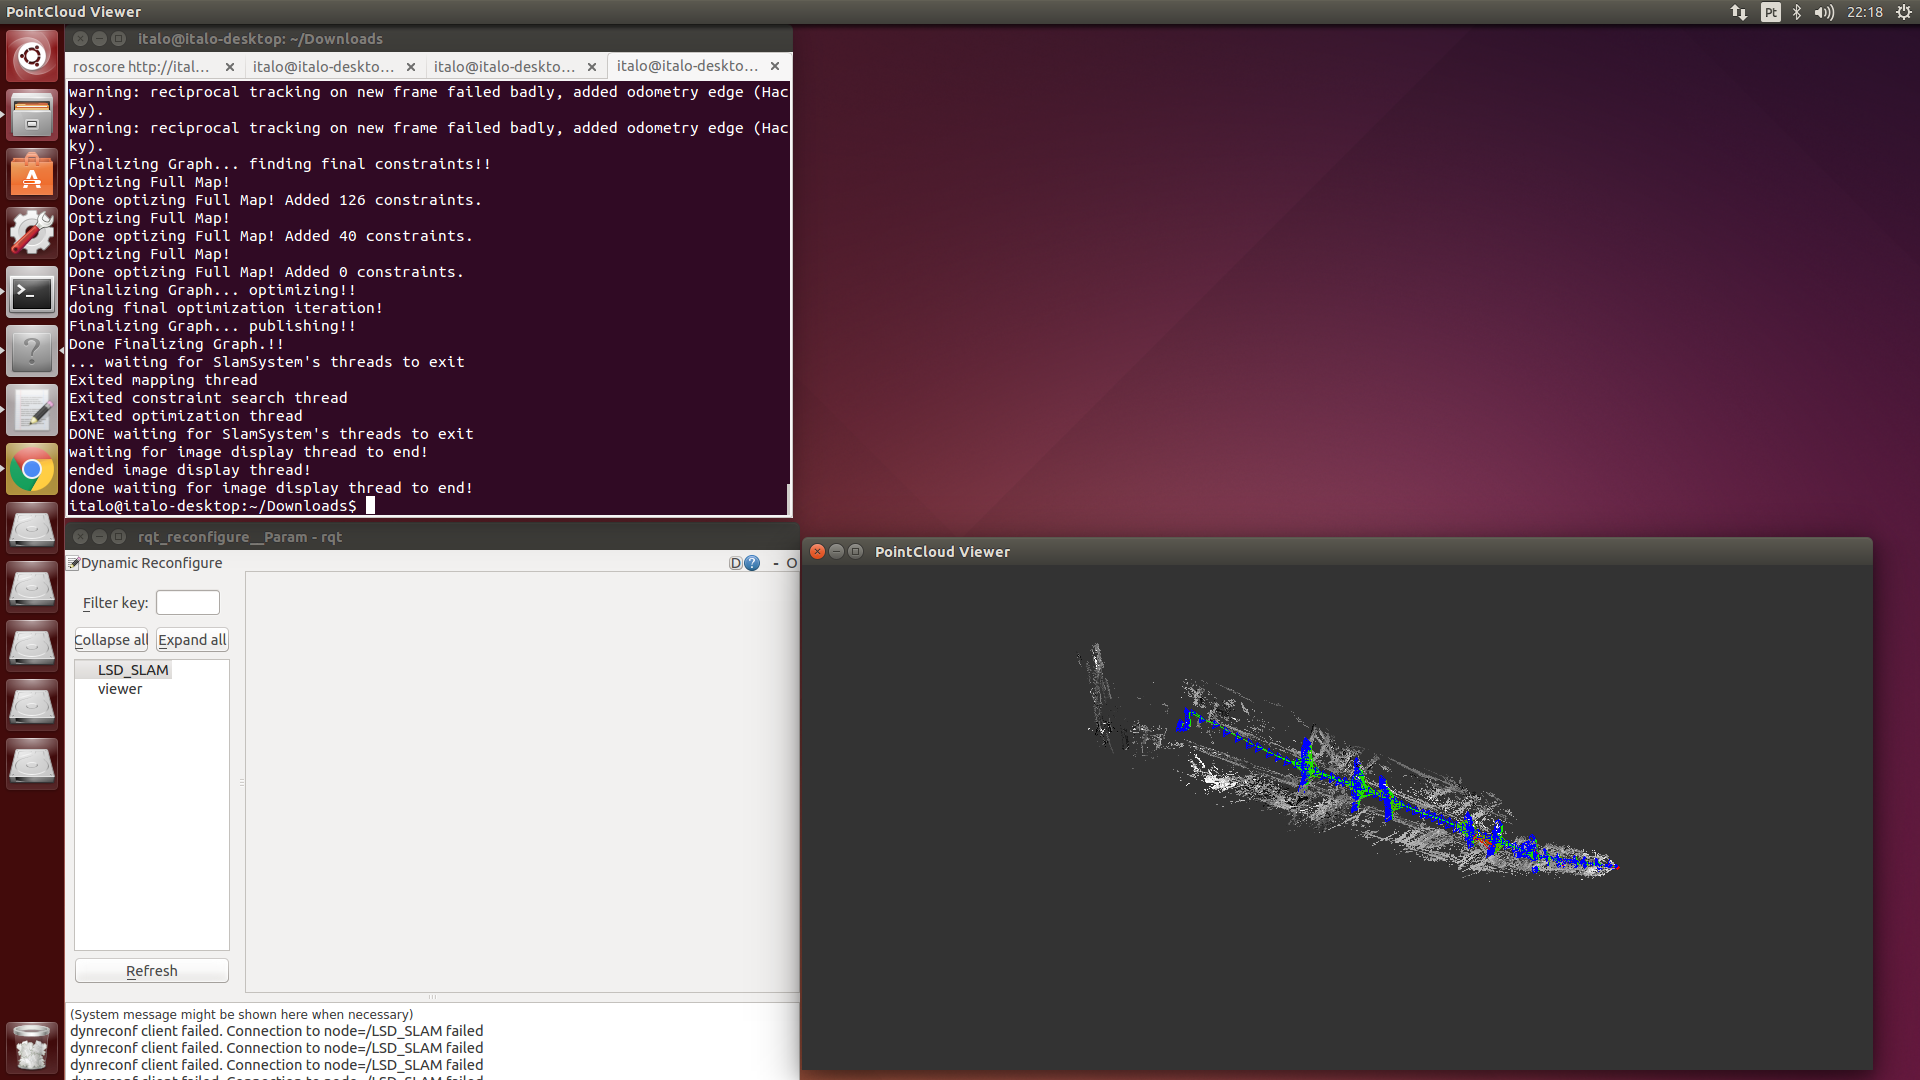
\includegraphics[width= \textwidth]{Imagens/figura3-40.png}
	\caption{\textit{PointCloud} e \textit{keyframes} do corredor do 1º andar do DCOMP usando o \textit{KFUsageWeight} e \textit{KFDistWeight} máximos de 20.0 \#1}
	\label{fig3:38}
\end{figure}

\begin{figure}[H]
	\centering
		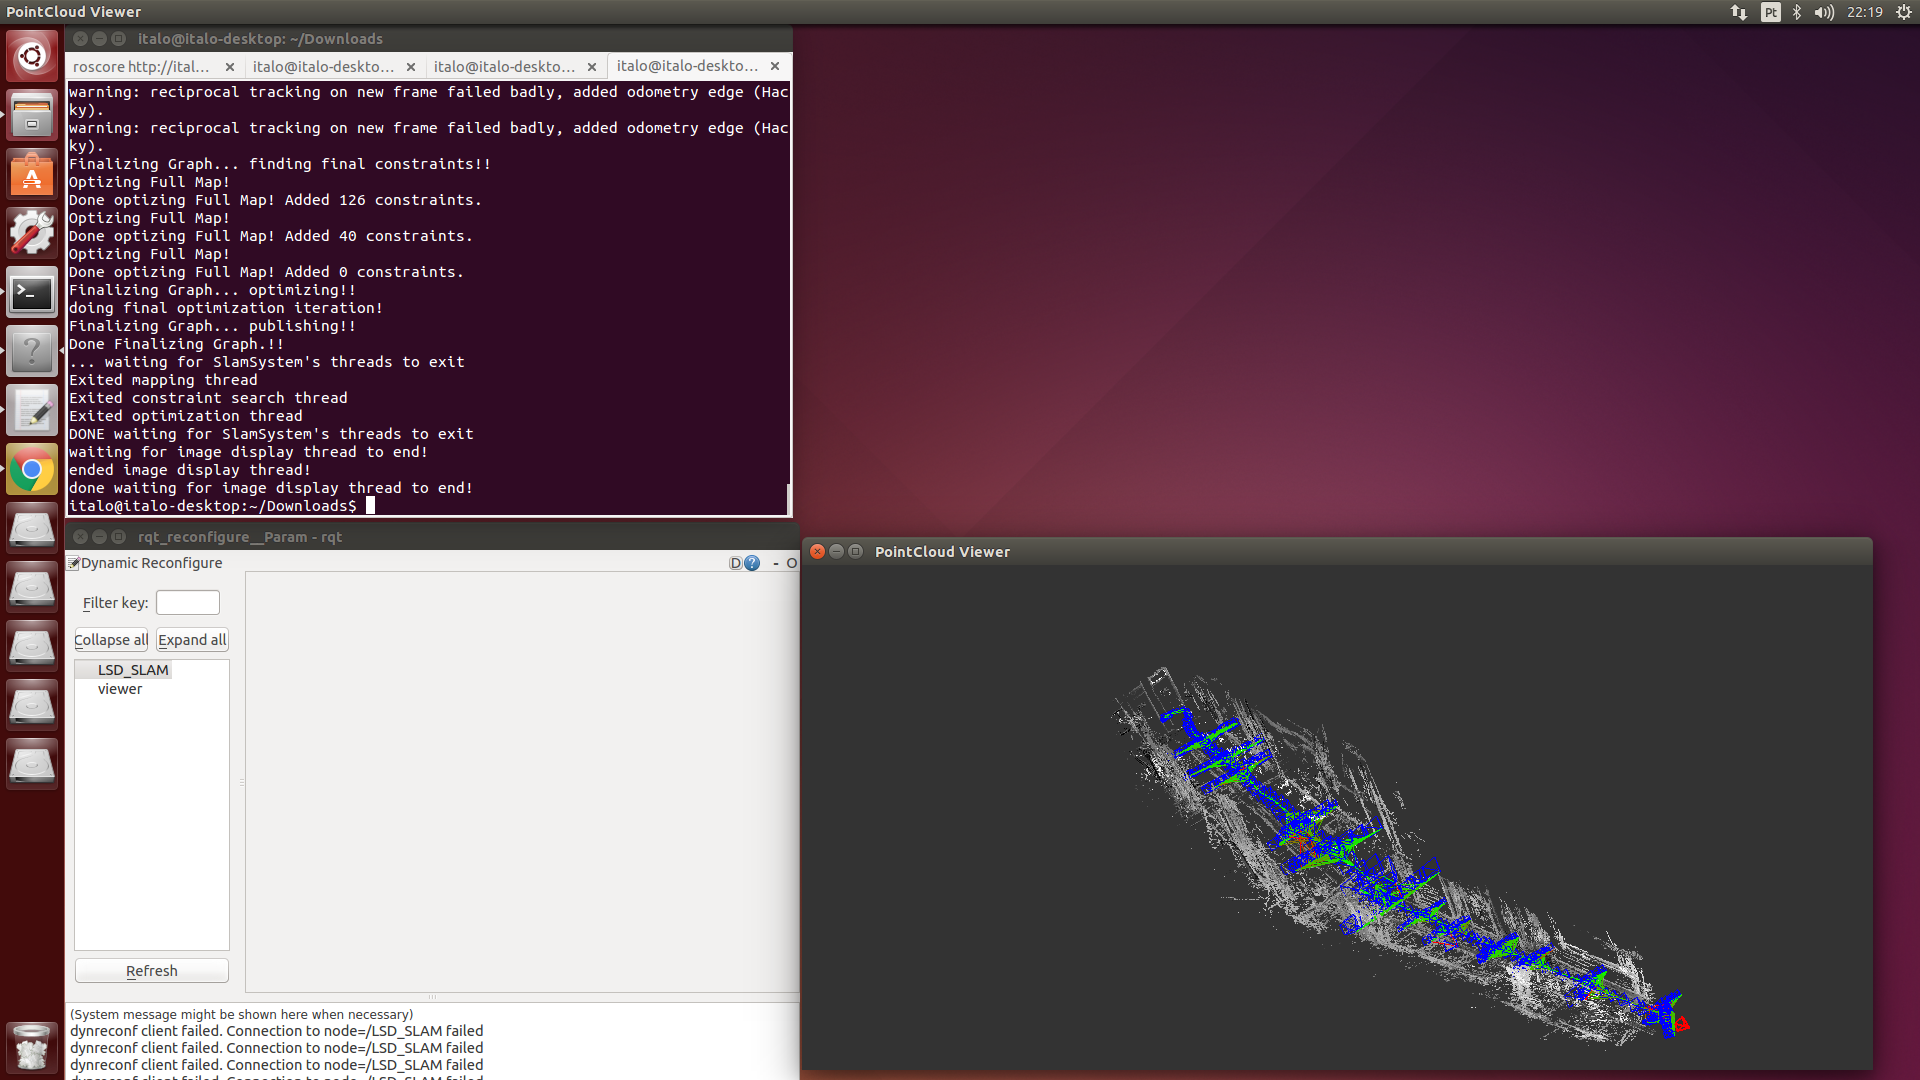
\includegraphics[width= \textwidth]{Imagens/figura3-41.png}
	\caption{\textit{PointCloud} e \textit{keyframes} do corredor do 1º andar do DCOMP usando o \textit{KFUsageWeight} e \textit{KFDistWeight} máximos de 20.0 \#2}
	\label{fig3:39}
\end{figure}